%!TEX root = ../exa-ma-d7.1.tex
\clearpage
\chapter{Software Frameworks powering Applications}
\label{chap:software}

This chapter presents the Exa-MA \emph{software frameworks} that power our applications—mini‑apps, extended mini‑apps, demonstrators, and proxy‑apps—using the terminology defined in Chapter~\ref{chap:methodology} (Structured Application Definitions). Each framework section briefly explains: (i) what the framework provides, (ii) which Exa‑MA Work Packages benefit, and (iii) which kinds of applications it enables in Chapter~\ref{chap:applications}.

We first provide general statistics across frameworks (architectures, languages, parallelism, I/O, DevOps). Then, we list the frameworks with concise capability summaries and pointers to their application entry points.

In the context of D7.1, we also clarify architectural capabilities (CPU/GPU/hybrid) to align with the benchmarking and CI/CD pipelines.

\paragraph{Application taxonomy (from methodology).}
Following Chapter~\ref{chap:methodology}:
\begin{description}
    \item[Mini‑app] Single kernel/algorithm focus (e.g., a preconditioner, mesh tool).
    \item[Extended mini‑app] Mini‑app with auxiliary scripts/data and I/O benchmarks.
    \item[Demonstrator] Integrated multi‑WP workflow for a scientific use‑case.
    \item[Proxy‑app] Representative full‑stack workload ($\geq 3$ WPs) for system tests.
\end{description}

\paragraph{Framework→Application links.}
For each framework below, we reference examples in Chapter~\ref{chap:applications} when available (e.g., Feel++ reduced‑basis mini‑apps, HPDDM‑enabled solver demonstrators, FreeFEM++ mesh‑adaptation extended mini‑apps).

The architectural capabilities benchmarked are classified as follows:

\paragraph{CPU Only}
Framework executes exclusively on CPUs (e.g., CGAL, FreeFEM++, Feel++, Manta). Benchmarks target CPU nodes.

\paragraph{GPU Only}
Framework executes exclusively on GPUs (e.g., Zellij). Benchmarks target GPU nodes.

\paragraph{CPU or GPU}
Framework can run on either CPU or GPU, but not concurrently within one run (e.g., PyTorch, SciMba). We benchmark both modes separately.

\paragraph{CPU and GPU}
Framework supports simultaneous CPU+GPU execution within a single run (e.g., TRUST). Benchmarks verify mixed‑architecture utilization.

\paragraph{Explanation of Benchmarking Criteria}
\begin{itemize}
    \item \textbf{CPU Only:} If selected, benchmarks will be performed exclusively on CPU architectures.
    \item \textbf{GPU Only:} If selected, benchmarks will focus exclusively on GPU architectures.
    \item \textbf{CPU and GPU:} If selected, benchmarks will involve simultaneous execution on CPU and GPU within the same run.
    \item \textbf{CPU or GPU:} If selected, benchmarks will involve execution on either CPU or GPU, but not simultaneously. Some benchmarks will target CPU, others GPU, depending on the computational components.
\end{itemize}


\section{General Statistics across Frameworks}
\label{sec:software:statistics}

In this section, we provide an overview of the key characteristics and technological choices for the software developed and benchmarked within Exa-MA. 
These statistics offer insights into the diversity of hardware architectures, programming languages, and parallel computing technologies utilized across the different software packages. 

The aim is to highlight the widespread usage of various technologies, demonstrating both the flexibility and the breadth of approaches within the project. 
Additionally, the DevOps practices employed, such as continuous integration, testing, and deployment, are presented to underscore the commitment to ensuring quality, reliability, and maintainability of the software developed under Exa-MA.

The following subsections show different aspects of the software frameworks involved in the project—supported architectures and programming languages, parallelism technologies, data formats, and DevOps strategies. This helps assess readiness for large‑scale simulations, CI/CD integration, and demonstrator pipelines.


\subsection{Architectures}

The following pie chart~\ref{fig:arch} shows the distribution of hardware architectures used for the benchmarks.

\begin{figure}[H]
\centering
\begin{tikzpicture}
\pie[text=legend, color={red, orange, yellow, lime}, sum=auto]{10/CPU Only, 5/CPU or GPU, 1/CPU and GPU, 2/GPU Only}
\end{tikzpicture}
\caption{Distribution of benchmarked hardware architectures}
\label{fig:arch}
\end{figure}


\subsection{Programming Languages}

The following pie chart~\ref{fig:languages} shows the distribution of programming languages used, highlighting the variety of computational solutions employed.

\begin{figure}[H]
\centering
\begin{tikzpicture}
\pie[text=legend, color={red, orange, yellow, lime, skyblue, pink, cyan, magenta}, sum=auto]{12/C++, 1/C\#, 2/C, 3/Fortran, 2/C++17, 5/Python, 1/C++20, 1/C++14}
\end{tikzpicture}
\caption{Distribution of programming languages}
\label{fig:languages}
\end{figure}


\subsection{Parallelism Technology}


The pie chart~\ref{fig:parallelism} below represents the parallelism techniques used in Exa-MA software selected for this document.

\begin{figure}[H]
\centering
\begin{tikzpicture}
\pie[text=legend, color={red, orange, yellow, lime, skyblue, pink}, sum=auto]{8/Multithread, 13/MPI, 8/GPU, 1/Parallelism - C++, 1/Task based, 1/Chapel}
\end{tikzpicture}
\caption{Distribution of parallelism technologies}
\label{fig:parallelism}
\end{figure}



\subsection{Data Formats}

The chart~\ref{fig:data} shows the supported data formats, for flexibility and compatibility in data handling, supported by Exa-MA software selected for this document.

\begin{figure}[H]
\centering
\begin{tikzpicture}
\pie[text=legend, color={red, orange, yellow, lime, skyblue, pink, cyan, magenta, peach, lavender}, sum=auto]{2/XML, 5/HDF5, 3/JSON, 2/Ensight, 5/None, 1/YAML, 1/Data-management system, 6/VTK, 5/in-house format, 4/Gmsh and associated formats, 2/MED, 1/MFront, 1/ASCII, 1/ROOT, 1/SQL}
\end{tikzpicture}
\caption{Distribution of data formats}
\label{fig:data}
\end{figure}


\subsection{Resilience}

The pie chart~\ref{fig:resilience} below shows the resilience mechanisms used in Exa-MA software selected for this document.

\begin{figure}[H]
\centering
\begin{tikzpicture}
\pie[text=legend, color={red}, sum=auto]{6/Checkpoint restart}
\end{tikzpicture}
\caption{Distribution of Resilience strategies}
\label{fig:resilience}
\end{figure}



\subsection{DevOps - CI/CD}

The pie chart~\ref{fig:devops-cicd} below displays the support of continuous integration and deployment practices as well as continuous benchmarking, showcasing systematic software updates, quality maintenance and performance regression.

\begin{figure}[H]
\centering
\begin{tikzpicture}
\pie[text=legend, color={red, orange, yellow, lime}, sum=auto]{11/Continuous Integration, 1/Continuous Benchmarking, 2/Continuous Delivery, 4/None}
\end{tikzpicture}
\caption{Distribution of DevOps CI/CD/CD}
\label{fig:devops-cicd}
\end{figure}


\subsection{DevOps - Packaging}

The next chart~\ref{fig:devops-packaging} shows different packaging methods used, which help in the distribution and management of software.

\begin{figure}[H]
\centering
\begin{tikzpicture}
\pie[text=legend, color={red, orange, yellow, lime, skyblue, pink}, sum=auto]{10/None, 5/Debian-based, 2/Fedora, 2/Spack, 1/GUIX, 1/Other}
\end{tikzpicture}
\caption{Distribution of DevOps Packaging}
\label{fig:devops-packaging}
\end{figure}


\subsection{DevOps - Containers}

The pie chart~\ref{fig:devops-containers} displays the use of container technologies, which help encapsulate the software to run reliably in various environments.

\begin{figure}[H]
\centering
\begin{tikzpicture}
\pie[text=legend, color={red, orange, yellow}, sum=auto]{12/None, 2/Apptainer/Singularity, 2/Docker}
\end{tikzpicture}
\caption{Distribution of DevOps Containers}
\label{fig:devops-containers}
\end{figure}


\subsection{DevOps - Testing}

The following pie chart~\ref{fig:devops-testing} details the testing practices adopted, illustrating the commitment to software reliability and functionality.

\begin{figure}[H]
\centering
\begin{tikzpicture}
\pie[text=legend, color={red, orange, yellow, lime, skyblue}, sum=auto]{9/Unit, 8/Verification, 4/Validation, 5/None, 1/Functional}
\end{tikzpicture}
\caption{Distribution of DevOps Testing}
\label{fig:devops-testing}
\end{figure}


% Framework descriptions (each subfile may also mention example mini‑apps/demonstrators)
%\section{Software: Arcane Framework}
\label{sec:Arcane Framework:software}



\begin{itemize}
    \item \textbf{Contact Email(s):} lydie.grospellier@cea.fr
    \item \textbf{Supported Architecture(s):} HYBRID
    \item \textbf{Repository Link:} \href{https://github.com/arcaneframework/framework}{https://github.com/arcaneframework/framework}
\end{itemize}

\subsection{Software summary}
\label{sec:Arcane Framework:summary}
Detailed overview not available.



\subsection{Purpose}
\label{sec:Arcane Framework:purpose}
Purpose not available.



\subsection{Mathematics}
\label{sec:Arcane Framework:mathematics}
Mathematics not available.


\subsection{Relevant Publications}
\label{sec:Arcane Framework:publications}

\subsection{Acknowledgements}
\label{sec::Arcane Framework:acknowledgements}

Acknowledgements not available.



\section{Software: CGAL}
\label{sec:CGAL:software}



\begin{itemize}
    \item \textbf{Contact Email(s):} pierre.alliez@inria.fr
    \item \textbf{Supported Architecture(s):} CPU
    \item \textbf{Repository Link:} \href{https://github.com/CGAL}{https://github.com/CGAL}
\end{itemize}

\subsection{Software summary}
\label{sec:CGAL:summary}
Detailed overview not available.



\subsection{Purpose}
\label{sec:CGAL:purpose}
Purpose not available.



\subsection{Mathematics}
\label{sec:CGAL:mathematics}
Mathematics not available.


\subsection{Relevant Publications}
\label{sec:CGAL:publications}

\subsection{Acknowledgements}
\label{sec::CGAL:acknowledgements}

Acknowledgements not available.



\section{Software: Composyx}
\label{sec:Composyx:software}

\begin{table}[h!]
    \centering
    { \setlength{\parindent}{0pt}
    \def\arraystretch{1.25}
    \arrayrulecolor{numpexgray}
    {\fontsize{9}{11}\selectfont
    \begin{tabular}{!{\color{numpexgray}\vrule}p{.4\textwidth}!{\color{numpexgray}\vrule}p{.6\textwidth}!{\color{numpexgray}\vrule}}
        \rowcolor{numpexgray}{\rule{0pt}{2.5ex}\color{white}\bf Field} & {\rule{0pt}{2.5ex}\color{white}\bf Details} \\
        \rowcolor{white}\textbf{Consortium} & \begin{tabular}{l}
None\\
\end{tabular} \\
        \rowcolor{numpexlightergray}\textbf{Exa-MA Partners} & \begin{tabular}{l}
Inria BXSO\\
\end{tabular} \\
        \rowcolor{white}\textbf{Contact Emails} & \begin{tabular}{l}
gilles.marait@inria.fr\\
\end{tabular} \\
        \rowcolor{numpexlightergray}\textbf{Supported Architectures} & \begin{tabular}{l}
CPU Only\\
\end{tabular} \\
        \rowcolor{white}\textbf{Repository} & \href{https://gitlab.inria.fr/composyx/composyx}{https://gitlab.inria.fr/composyx/composyx} \\
        \rowcolor{numpexlightergray}\textbf{License} & \begin{tabular}{l}
OSS: Cecill-*\\
\end{tabular} \\
        \rowcolor{white}\textbf{Bottlenecks roadmap} & \begin{tabular}{l}
B10 - Scientific Productivity\\
B11 - Reproducibility and Replicability of Computation\\
B6 - Data Management\\
B7 - Exascale Algorithms\\
\end{tabular} \\
        \bottomrule
    \end{tabular}
    }}
    \caption{Composyx Information}
\end{table}

\subsection{Software summary}
\label{sec:Composyx:summary}
Composyx (previously  Maphys++) is a linear algebra C++20 library focused on composability. Its purpose is to allow the user to express a large panel of algorithms using a high-level interface to range from laptop prototypes to many node supercomputer parallel computations.
Currently it mostly implements domain decomposition methods as described in~\cite{agullo_robust_2019} using hybrid parallel implementation (MPI+Thread, MPI+StarPU) to address heterogeneous manycores.

\begin{figure}
        \centering
        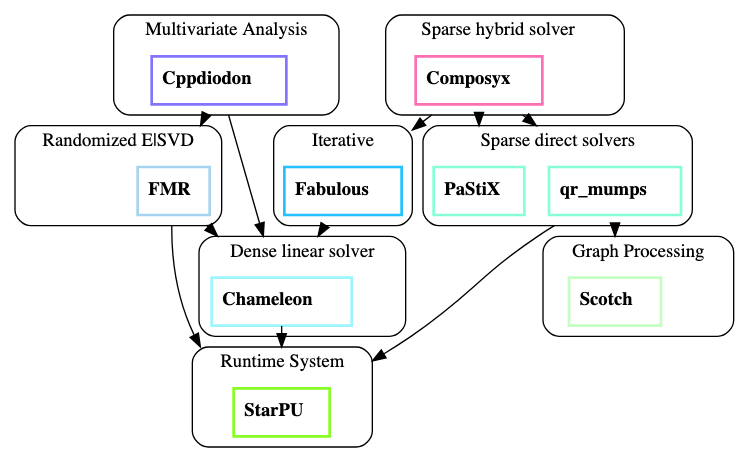
\includegraphics[width=0.8\textwidth]{graphics/composyx/composyx-solverstack.png}
        \caption{Composyx dependencies}
        \label{fig:composyx}
    \end{figure}

\subsection{Purpose}
\label{sec:Composyx:purpose}
Solution of large sparse linear systems using preconditioned subspace methods. For that purpose it relies on the Fabulous packages that implements various techniques including block variants for multiple right-hand sides~\cite{giraud_block_2022}.

\subsection{Programming and Computational Environment}
\label{sec::Composyx:environment_capabilities}


The following table summarizes these aspects for Composyx, providing a  view of its programming and computational capabilities.

\begin{table}[h!]
    \centering
    {
    \setlength{\parindent}{0pt}
    \def\arraystretch{1.25}
    \arrayrulecolor{numpexgray}
    {\fontsize{9}{11}\selectfont
    \begin{tabular}{lp{.3\textwidth}p{.5\textwidth}}
        \rowcolor{numpexgray}{\rule{0pt}{2.5ex}\color{white}\bf Category}  & {\rule{0pt}{2.5ex}\color{white}\bf Details} & {\rule{0pt}{2.5ex}\color{white}\bf Description}\\
        \rowcolor{white}Languages  & \begin{tabular}{l}
C\\
C++20\\
Fortran\\
\end{tabular} & Programming languages and language standards supported by the software \\
        \rowcolor{numpexlightergray}Parallelism  & \begin{tabular}{l}
GPU\\
MPI\\
Multithread\\
\end{tabular} & Parallel computing methods and frameworks utilized by the software.\\
        \rowcolor{white}Data Formats  & \begin{tabular}{l}
None\\
\end{tabular} & Data formats that the software can handle or produce.\\
        \rowcolor{numpexlightergray}Resilience  & \begin{tabular}{l}
None\\
\end{tabular} & Fault tolerance and recovery mechanisms employed by the software.\\
        \rowcolor{white}DevOps & \begin{tabular}{l}
Continuous Integration\\
\end{tabular} & Outlines the development and operational practices including continuous integration, containerization, and testing methodologies.  \\
        \rowcolor{numpexlightergray}Packaging  & \begin{tabular}{l}
GUIX-HPC\\
\end{tabular} & Software packaging and distribution.\\
        \rowcolor{white}Testing  & \begin{tabular}{l}
Verification\\
\end{tabular} & Testing methodologies employed to ensure software quality and correctness.\\
        \rowcolor{numpexlightergray}Containerization  & \begin{tabular}{l}
Singularity\\
\end{tabular} & Container technologies used to package and deploy the software.\\
        \rowcolor{white}Interfaces  & \begin{tabular}{l}
MUMPS\\
PaStiX\\
Scotch\\
qr\_mumps\\
\end{tabular} & List of software Composyx has interfaces with.\\
        \bottomrule
    \end{tabular}
    }}
    \caption{Composyx programming and computational environment}
\end{table}



%\subsection{Mathematics}
%\label{sec:Composyx:mathematics}
%Mathematics not available.

%In this section, provide a summary the mathematics used in the software.


\subsection{Relevant Publications}
\label{sec:Composyx:publications}

Here is a list of relevant publications related to the software:
\begin{description}
        \item[\fullcite{agullo_robust_2019}]
        The solution of large sparse linear systems is one of the most time consuming kernels in many numerical simulations. The domain decomposition community has developed many efficient and robust methods in the last decades. While many of these solvers fall into the abstract Schwarz (aS) framework, their robustness was originally demonstrated on a case-by-case basis. In this paper, we propose a bound for the condition number of all deflated aS methods provided that the coarse grid consists of the assembly of local components that contain the kernel of some local operators. We show that classical results from the literature on particular instances of aS methods can be retrieved from this bound. We then show that such a coarse grid correction can be explicitly obtained algebraically via generalized eigenproblems, leading to a condition number independent of the number of domains. This result can be readily applied to retrieve or improve the bounds previously obtained via generalized eigenproblems in the particular cases of Neumann-Neumann (NN), additive Schwarz (AS), and optimized Robin, but it also generalizes them when applied with approximate local solvers. Interestingly, the proposed methodology turns out to be a comparison of the considered particular aS method with generalized versions of both NN and AS for tackling the lower and upper part of the spectrum, respectively. We furthermore show that the application of the considered grid corrections in an additive fashion is robust in the AS case although it is not robust for aS methods in general. In particular, the proposed framework allows for ensuring the robustness of the AS method applied on the Schur complement, either with deflation or additively, and with the freedom of relying on an approximate local Schur complement. Numerical experiments illustrate these statements.
    \item[\fullcite{agullo_soft_2020}]
    The conjugate gradient (CG) method is the most widely used iterative scheme for the solution of large sparse systems of linear equations when the matrix is symmetric positive definite. Although more than 60 years old, it is still a serious candidate for extreme-scale computations on large computing platforms. On the technological side, the continuous shrinking of transistor geometry and the increasing complexity of these devices affect dramatically their sensitivity to natural radiation and thus diminish their reliability. One of the most common effects produced by natural radiation is the single event upset which consists in a bit-flip in a memory cell producing unexpected results at the application level. Consequently, future extreme-scale computing facilities will be more prone to errors of any kind, including bit-flips, during their calculations. These numerical and technological observations are the main motivations for this work, where we first investigate through extensive numerical experiments the sensitivity of CG to bit-flips in its main computationally intensive kernels, namely the matrix-vector product and the preconditioner application. We further propose numerical criteria to detect the occurrence of such soft errors and assess their robustness through extensive numerical experiments.
    \item[\fullcite{giraud_block_2022}]
        We are concerned with the iterative solution of linear systems with multiple right-hand sides available one group after another with possibly slowly varying left-hand sides. For such sequences of linear systems, we first develop a new block minimum norm residual approach that combines two main ingredients. The first component exploits ideas from GCRO-DR~\cite{parks_recycling_2006}, enabling us to recycle information from one solve to the next. The second component is the numerical mechanism for managing the partial convergence of the right-hand sides, referred to as inexact breakdown detection in IB-BGMRES~\cite{robbe_exact_2006}, that enables the monitoring of the rank deficiency in the residual space basis expanded blockwise. Next, for the class of block minimum norm residual approaches that relies on a block Arnoldi-like equality between the search space and the residual space (e.g., any block GMRES or block GCRO variants), we introduce new search space expansion policies defined on novel criteria to detect the partial convergence. These novel detection criteria are tuned to the selected stopping criterion and targeted convergence threshold to best cope with the selected normwise backward error stopping criterion, enabling us to monitor the computational effort while ensuring the final accuracy of each individual solution. Numerical experiments are reported to illustrate the numerical and computational features of both the new block Krylov solvers and the new search space block expansion polices.
\end{description}

\subsection{Acknowledgements}
\label{sec::Composyx:acknowledgements}

The software has been developed with the support of the following funding agencies and institutions: 




Acknowledgements not available.



%!TEX root = ../../exa-ma-d7.1.tex
\section{Software: \texorpdfstring{\Feelpp}{Feel++}}
\label{sec:Feelpp:software}

\begin{table}[!ht]
    \centering
    { \setlength{\parindent}{0pt}
    \def\arraystretch{1.25}
    \arrayrulecolor{numpexgray}
    {\fontsize{9}{11}\selectfont
    \begin{tabular}{!{\color{numpexgray}\vrule}p{.4\textwidth}!{\color{numpexgray}\vrule}p{.6\textwidth}!{\color{numpexgray}\vrule}}
        \rowcolor{numpexgray}{\rule{0pt}{2.5ex}\color{white}\bf Field} & {\rule{0pt}{2.5ex}\color{white}\bf Details} \\
        \rowcolor{white}\textbf{Consortium} & \begin{tabular}{l}
\Feelpp Consortium\\
\end{tabular} \\
        \rowcolor{numpexlightergray}\textbf{Exa-MA Partners} & \begin{tabular}{l}
CNRS\\
Inria Grenoble\\
Unistra\\
\end{tabular} \\
        \rowcolor{white}\textbf{Contact Emails} & \begin{tabular}{l}
christophe.prudhomme@cemosis.fr\\
vincent.chabannes@cemosis.fr\\
\end{tabular} \\
        \rowcolor{numpexlightergray}\textbf{Supported Architectures} & \begin{tabular}{l}
CPU Only\\
\end{tabular} \\
        \rowcolor{white}\textbf{Repository} & \href{https://github.com/feelpp/feelpp}{https://github.com/feelpp/feelpp} \\
        \rowcolor{numpexlightergray}\textbf{License} & \begin{tabular}{l}
OSS:: GPL v*\\
OSS:: LGPL v*\\
\end{tabular} \\
        \rowcolor{white}\textbf{Bottlenecks roadmap} & \begin{tabular}{l}
B10 - Scientific Productivity\\
B11 - Reproducibility and Replicability of Computation\\
B12 - Pre/Post Processing and In-Situ Processing\\
B2 - Interconnect Technology\\
B6 - Data Management\\
B7 - Exascale Algorithms\\
\end{tabular} \\
        \hline
    \end{tabular}
    }}
    \caption{\Feelpp Information}
\end{table}

\subsection{Software summary}
\label{sec:Feelpp:summary}

\feelpp is a powerful framework designed to solve problems based on ordinary differential equations (ODEs) and partial differential equations (PDEs).
It leverages modern \Cpp{} standards, including \Cpp{17} and \Cpp{20}, and also provides a Python layer through Pybind11.
The suite is particularly effective for parallel computing, with seamless integration of parallelism through default communicators, including support for ensemble runs.



\Feelpp provides several specialized toolboxes to address various fields of numerical simulation
\begin{inparaenum}[(i)]
        \item fluid mechanics,
        \item solid mechanics,
        \item heat transfer and conjuguate heat transfer,
        \item fluid structure interaction,
        \item electro and magnetostatic,
        \item thermoelectric,
        \item levelset and multifluid.
\end{inparaenum}
Each toolbox is tailored to specific types of problems, ensuring high performance and accuracy.

\Feelpp is used in a variety of fields, particularly in health, industry, and physics. Below are some examples of applications:
\begin{inparaenum}[(i)]
    \item \textbf{Health (Brain)}: Applications related to brain modeling.
    \item \textbf{Health (Tumor Cells)}: Simulation of tumor cell behavior.
    \item \textbf{Industry (ROM, UQ)}: Reduced-order modeling and uncertainty quantification in industrial settings.
    \item \textbf{Automotive (CFD, ROM)}: Computational fluid dynamics and reduced-order models in automotive engineering.
    \item \textbf{Physics (High Field Magnets)}: Simulations of high field magnets.
    \item \textbf{Health (Rheology)}: Modeling blood rheology.
    \item \textbf{Health (Eye/Brain)}: Coupling between the eye and the brain in medical simulations.
\end{inparaenum}

The \Feelpp core library provides a wide range of numerical methods for solving PDEs, with support for finite elements in various Sobolev spaces with scalar, vector and matrix values. For example:
\begin{inparaenum}[(i)]
    \item \( L^2 \), \( \mathbf{L}^2 \), \( \mathbb{L}^2 \)
    \item \( H^1 \), \( \mathbf{H}^1 \), \( \mathbb{H}^1 \)
    \item \( \mathbf{H}(\text{div}) \), \( \mathbf{H}(\text{curl}) \)
\end{inparaenum}

\Feelpp supports a wide variety of element types and value types, including single, double, and quad precision, as well as complex numbers. The supported problem domains include 0D to 3D, with or without time dependence.

Here is a typical example of solving a Laplace equation in \Feelpp:

\begin{listing}[ht]
        \caption{Sample \Feelpp code for solving a Laplace equation on an arbitrary domain.}
\begin{minted}[
        linenos,                % Line numbers
        fontsize=\scriptsize,        % Reduce font size
        bgcolor=bgcolor,        % Slightly gray background
        frame=lines,            % Delimiters around the code
        framesep=2mm,           % Space between code and frame
        rulecolor=\color{gray}, % Color of the frame
        breaklines              % Allow line breaks in long lines
      ]{cpp}
auto Vh = Pch<4>(mesh, markedelements(mesh, expr("<...>")));
auto u = Vh->element(), v = Vh->element(g, "g");
auto l = form1(_test = Vh);
l = integrate(_range = elements(support(Vh)), _expr = f * id(v));
l += integrate(_range = markedfaces(support(Vh), "Robin"), _expr = -r_2 * id(v));
l += integrate(_range = markedfaces(support(Vh), "Neumann"), _expr = -un * id(v));

auto a = form2(_trial = Vh, _test = Vh);
a = integrate(_range = elements(support(Vh)), _expr = inner(k * gradt(u), grad(v)));
a += integrate(_range = markedfaces(support(Vh), "Robin"), _expr = r_1 * idt(u) * id(v));
a += on(_range = markedfaces(support(Vh), "Dirichlet"), _rhs = l, _element = u, _expr = g);
a.solve(_rhs = l, _solution = u);
\end{minted}
\end{listing}

The suite supports multiple linear algebra libraries, including PETSc, SLEPc, Eigen, and Boost::ublas, and is designed to run efficiently in both sequential and parallel environments.



\Feelpp is a versatile and powerful tool for solving PDEs and ODEs in a variety of scientific and industrial applications.
With support for high-performance computing and a broad range of numerical methods which can be used to build taylored applications for research, development, and teaching.


\subsection{Purpose}
\label{sec:Feelpp:purpose}
\Feelpp aims to provide a flexible and efficient environment for conducting finite element analysis in multiple scientific domains.
It allows for the rapid prototyping of numerical models and is built with parallel computing in mind to scale on modern HPC architectures.

\subsection{Programming and Computational Environment}
\label{sec::Feelpp:environment_capabilities}

The~\Cref{tab:Feelpp:environment_capabilities} summarizes these aspects for \Feelpp, providing a view of its programming and computational capabilities.

%% \begin{table}[!ht]
%% %%    \centering
%%     {
%%     \setlength{\parindent}{0pt}
%%     \def\arraystretch{1.25}
%%     \arrayrulecolor{numpexgray}
%%     {\fontsize{9}{11}\selectfont
%%     \begin{longtable}{lp{.3\textwidth}p{.5\textwidth}}
%%         \rowcolor{gray}\textbf{\color{white}Category} & \textbf{\color{white}Details} & \textbf{\color{white}Description} \\
%%         \hline
%%         \endfirsthead % End of the first head (the header for the first page)
%%
%%         \hline
%%         \rowcolor{gray}\textbf{Category} & \textbf{Details} & \textbf{Description} \\
%%         \hline
%%         \endhead % End of the head (for all other pages)
%%
%%         \hline
%%         \endfoot % Footer for all but the last page
%%
%%         \hline
%%         \endlastfoot % Footer for the last page
%%
%%         \rowcolor{white}Languages  & \begin{tabular}{l}
%% C++\\
%% C++17\\
%% C++20\\
%% Python\\
%% \end{tabular} & \Feelpp is primarily developed in C++ and supports modern C++ standards, including C++17 and C++20, which provide enhanced performance, safety features, and modern programming paradigms for high-performance computing applications. This allows \Feelpp to leverage advanced language features such as constexpr, parallel algorithms, and enhanced lambda expressions, improving both code maintainability and computational efficiency. Additionally, \Feelpp integrates with Python, enabling scripting capabilities and facilitating ease of use for rapid prototyping, automation, and integration with scientific workflows. This dual-language support provides flexibility for both performance-critical tasks and user-friendly interfaces. \\
%%         \rowcolor{numpexlightergray}Parallelism  & \begin{tabular}{l}
%% MPI\\
%% Parallelism - C++\\
%% Task based\\
%% \end{tabular} & \Feelpp offers robust support for parallel computing, making it suitable for high-performance simulations. It utilizes MPI (Message Passing Interface) for distributed memory parallelism, enabling efficient communication between processes across different nodes in HPC environments. Additionally, \Feelpp implements parallelism directly in C++, allowing fine-grained control over threading and parallel execution within shared memory systems. The framework also supports task-based parallelism thanks to specx, enabling the efficient execution of independent computational tasks, improving load balancing, and optimizing resource usage across heterogeneous computing architectures. This parallelism support ensures scalability and high performance in complex multiphysics simulations.\\
%%         \rowcolor{white}Data Formats  & \begin{tabular}{l}
%% Data-management system\\
%% Ensight\\
%% Gmsh and associated formats\\
%% HDF5\\
%% JSON\\
%% VTK\\
%% YAML\\
%% in-house format\\
%% \end{tabular} & \Feelpp supports data management, including remote data management systems such as Girder and GitHub. It handles a variety of input and output formats, including Ensight, Gmsh, HDF5, JSON, VTK, YAML, and an in-house format. This flexibility enables \Feelpp to align with the \textbf{FAIR} principles (Findable, Accessible, Interoperable, and Reusable), ensuring efficient data sharing and reuse across different platforms and tools.\\
%%         \rowcolor{numpexlightergray}Resilience  & \begin{tabular}{l}
%% Checkpoint restart\\
%% \end{tabular} & \Feelpp provides resilience support through checkpoint restart functionality. This allows simulations to save their state at specific points, enabling recovery from failures without restarting from the beginning. Binary in-house formats are used for fast restarts, ensuring minimal downtime and efficient continuation of long-running computations, especially on large-scale HPC systems.\\
%%         \rowcolor{white}DevOps & \begin{tabular}{l}
%% Continuous Benchmarking\\
%% Continuous Delivery\\
%% Continuous Integration\\
%% \end{tabular} & Outlines the development and operational practices including continuous integration, containerization, and testing methodologies.  \\
%%         \rowcolor{numpexlightergray}Packaging  & \begin{tabular}{l}
%% Debian\\
%% Fedora\\
%% Spack\\
%% Ubuntu\\
%% \end{tabular} & \Feelpp is available in various packaging formats to ensure broad compatibility across different platforms. It is packaged for popular Linux distributions and HPC environments, with specific mirrors and repositories:\\
%%         \rowcolor{white}Testing  & \begin{tabular}{l}
%% Unit\\
%% Validation\\
%% Verification\\
%% \end{tabular} & Testing methodologies employed to ensure software quality and correctness.\\
%%         \rowcolor{numpexlightergray}Containerization  & \begin{tabular}{l}
%% Docker\\
%% Singularity\\
%% \end{tabular} & Container technologies used to package and deploy the software.\\
%%         \rowcolor{white}Interfaces  & \begin{tabular}{l}
%% Dymola/OpenModelica/FMU\\
%% HPdomain decomposition methods\\
%% MMG/ParMMG\\
%% OpenTurns\\
%% PETSc\\
%% Salome\\
%% \end{tabular} & List of software \Feelpp has interfaces with.\\
%%         \bottomrule
%%     \end{longtable}
%%     }}
%%     \caption{\Feelpp programming and computational environment}
%% \end{table}

{\fontsize{9}{11}\selectfont
\begin{longtable}{lp{0.3\textwidth}p{0.5\textwidth}}
        \caption{\Feelpp programming and computational environment}\label{tab:Feelpp:environment_capabilities} \\
        \rowcolor{gray}\textbf{\color{white}Category} & \textbf{\color{white}Details} & \textbf{\color{white}Description} \\
        \hline
        \endfirsthead % End of the first head (the header for the first page)

        \hline
        \rowcolor{gray}\textbf{\color{white}Category} & \textbf{\color{white}Details} & \textbf{\color{white}Description} \\
        \hline
        \endhead % End of the head (for all other pages)

        \hline
        \endfoot % Footer for all but the last page

        \hline
        \endlastfoot % Footer for the last page

        \rowcolor{white}Languages  & \begin{tabular}{l}
                \Cpp{}\\
                \Cpp{17}\\
                \Cpp{20}\\
                Python\\
                \end{tabular} & \Feelpp is primarily developed in \Cpp{} and supports modern \Cpp{} standards, including \Cpp{17} and \Cpp{20}, which provide enhanced performance and safety features for high-performance computing applications. It also integrates with Python for scripting capabilities. \\

        \rowcolor{numpexlightergray}Parallelism  & \begin{tabular}{l}
                MPI\\
                Parallelism - \Cpp{}\\
                Task based\\
                \end{tabular} & \Feelpp offers robust support for parallel computing, utilizing MPI for distributed memory parallelism and implementing task-based parallelism to improve load balancing and resource usage. \\

        \rowcolor{white}Data Formats  & \begin{tabular}{l}
                Data-management system\\
                Ensight\\
                Gmsh and associated formats\\
                HDF5\\
                JSON\\
                VTK\\
                YAML\\
                in-house format\\
                \end{tabular} & \Feelpp supports various data formats for efficient data sharing and reuse, aligning with the FAIR principles. \\

        \rowcolor{numpexlightergray}Resilience  & Checkpoint restart & \Feelpp provides resilience support through checkpoint restart functionality. This allows simulations to save their state at specific points, enabling recovery from failures without restarting from the beginning. Binary in-house formats are used for fast restarts, ensuring minimal downtime and efficient continuation of long-running computations, especially on large-scale HPC systems.\\

        \rowcolor{white}DevOps & \begin{tabular}{l} Continuous Benchmarking\\
                Continuous Delivery\\
                Continuous Integration\\
                \end{tabular} & \Feelpp is developped on GitHub and uses GitHub Actions workflows to ensure the quality of the developments. The main branch is protected and only accepted reviewed PR can be merged. \Feelpp is not only rebuilt by the CI but also tests are run.  Upon merge, a packaging workflow is trigerred to generate Debian-based packages as well as Docker and Apptainer images. Once Apptainer images are available, benchmarks are trigerred on super computer to check the performances, see~\cref{fig:feelpp-ci} and~\cref{fig:feelpp-cb} for a graphical representation.\\

        \rowcolor{numpexlightergray}Packaging  & Debian, Fedora, Spack, Ubuntu & Debian-based systems: Available via the APT repository at \href{https://apt.feelpp.org}{apt.feelpp.org}. Detailed installation instructions can be found in the documentation: \href{https://docs.feelpp.org/user/latest/install/index.html}{\Feelpp Installation Guide}.
        Fedora: Distributed via Docker images, simplifying deployment in containerized environments.
        Spack: Supported by Spack for high-performance computing environments, with a mirror available at \href{https://ghcr.io/feelpp/spack}{ghcr.io/feelpp/spack}.
        Ubuntu: Also available through the same APT repository for Debian-based systems.\\

        \rowcolor{white}Testing  & \begin{tabular}{l}
                Unit\\
                Validation\\
                Verification\\
                \end{tabular} & \Feelpp includes a suite of nearly 1,000 tests executed via ctest. These tests correspond to applications run both sequentially and in parallel. In most cases, applications are tested in both modes; only on very rare occasions are they run exclusively in either sequential or parallel mode. Each application contains numerous tests that perform unit testing or verify expected mathematical properties. To detect excessive execution time regressions, timeouts are configured for the tests. Finally, some tests are mini-applications or benchmarks that perform verification or validation against reference results.\\

        \rowcolor{numpexlightergray}Containerization  & Docker, Singularity & \Feelpp supports Docker and Apptainer/Singularity containers built either from source or from Debian-based packages. Both container type images are stored on \url{https://ghcr.io/feelpp/feelpp}. Images with tags containing \texttt{-sif} appended are apptainer images, the other ones are docker images. \\

        \rowcolor{white}Interfaces  &\begin{tabular}{l}
                Dymola/OpenModelica/FMU\\
                hpddm\\
                MMG/ParMMG\\
                OpenTurns\\
                PETSc\\
                Salome\\
                CGAL\\
                Scimba
                \end{tabular} & \Feelpp can easily be interfaced with various software thanks to the use of standard open formats and a flexible \Cpp{} design.\\


    \end{longtable}
    }



    The~\Cref{fig:feelpp-ci} shows the \Feelpp Continuous Integration Workflow using GitHub Actions.
    \begin{figure}
        \centering
        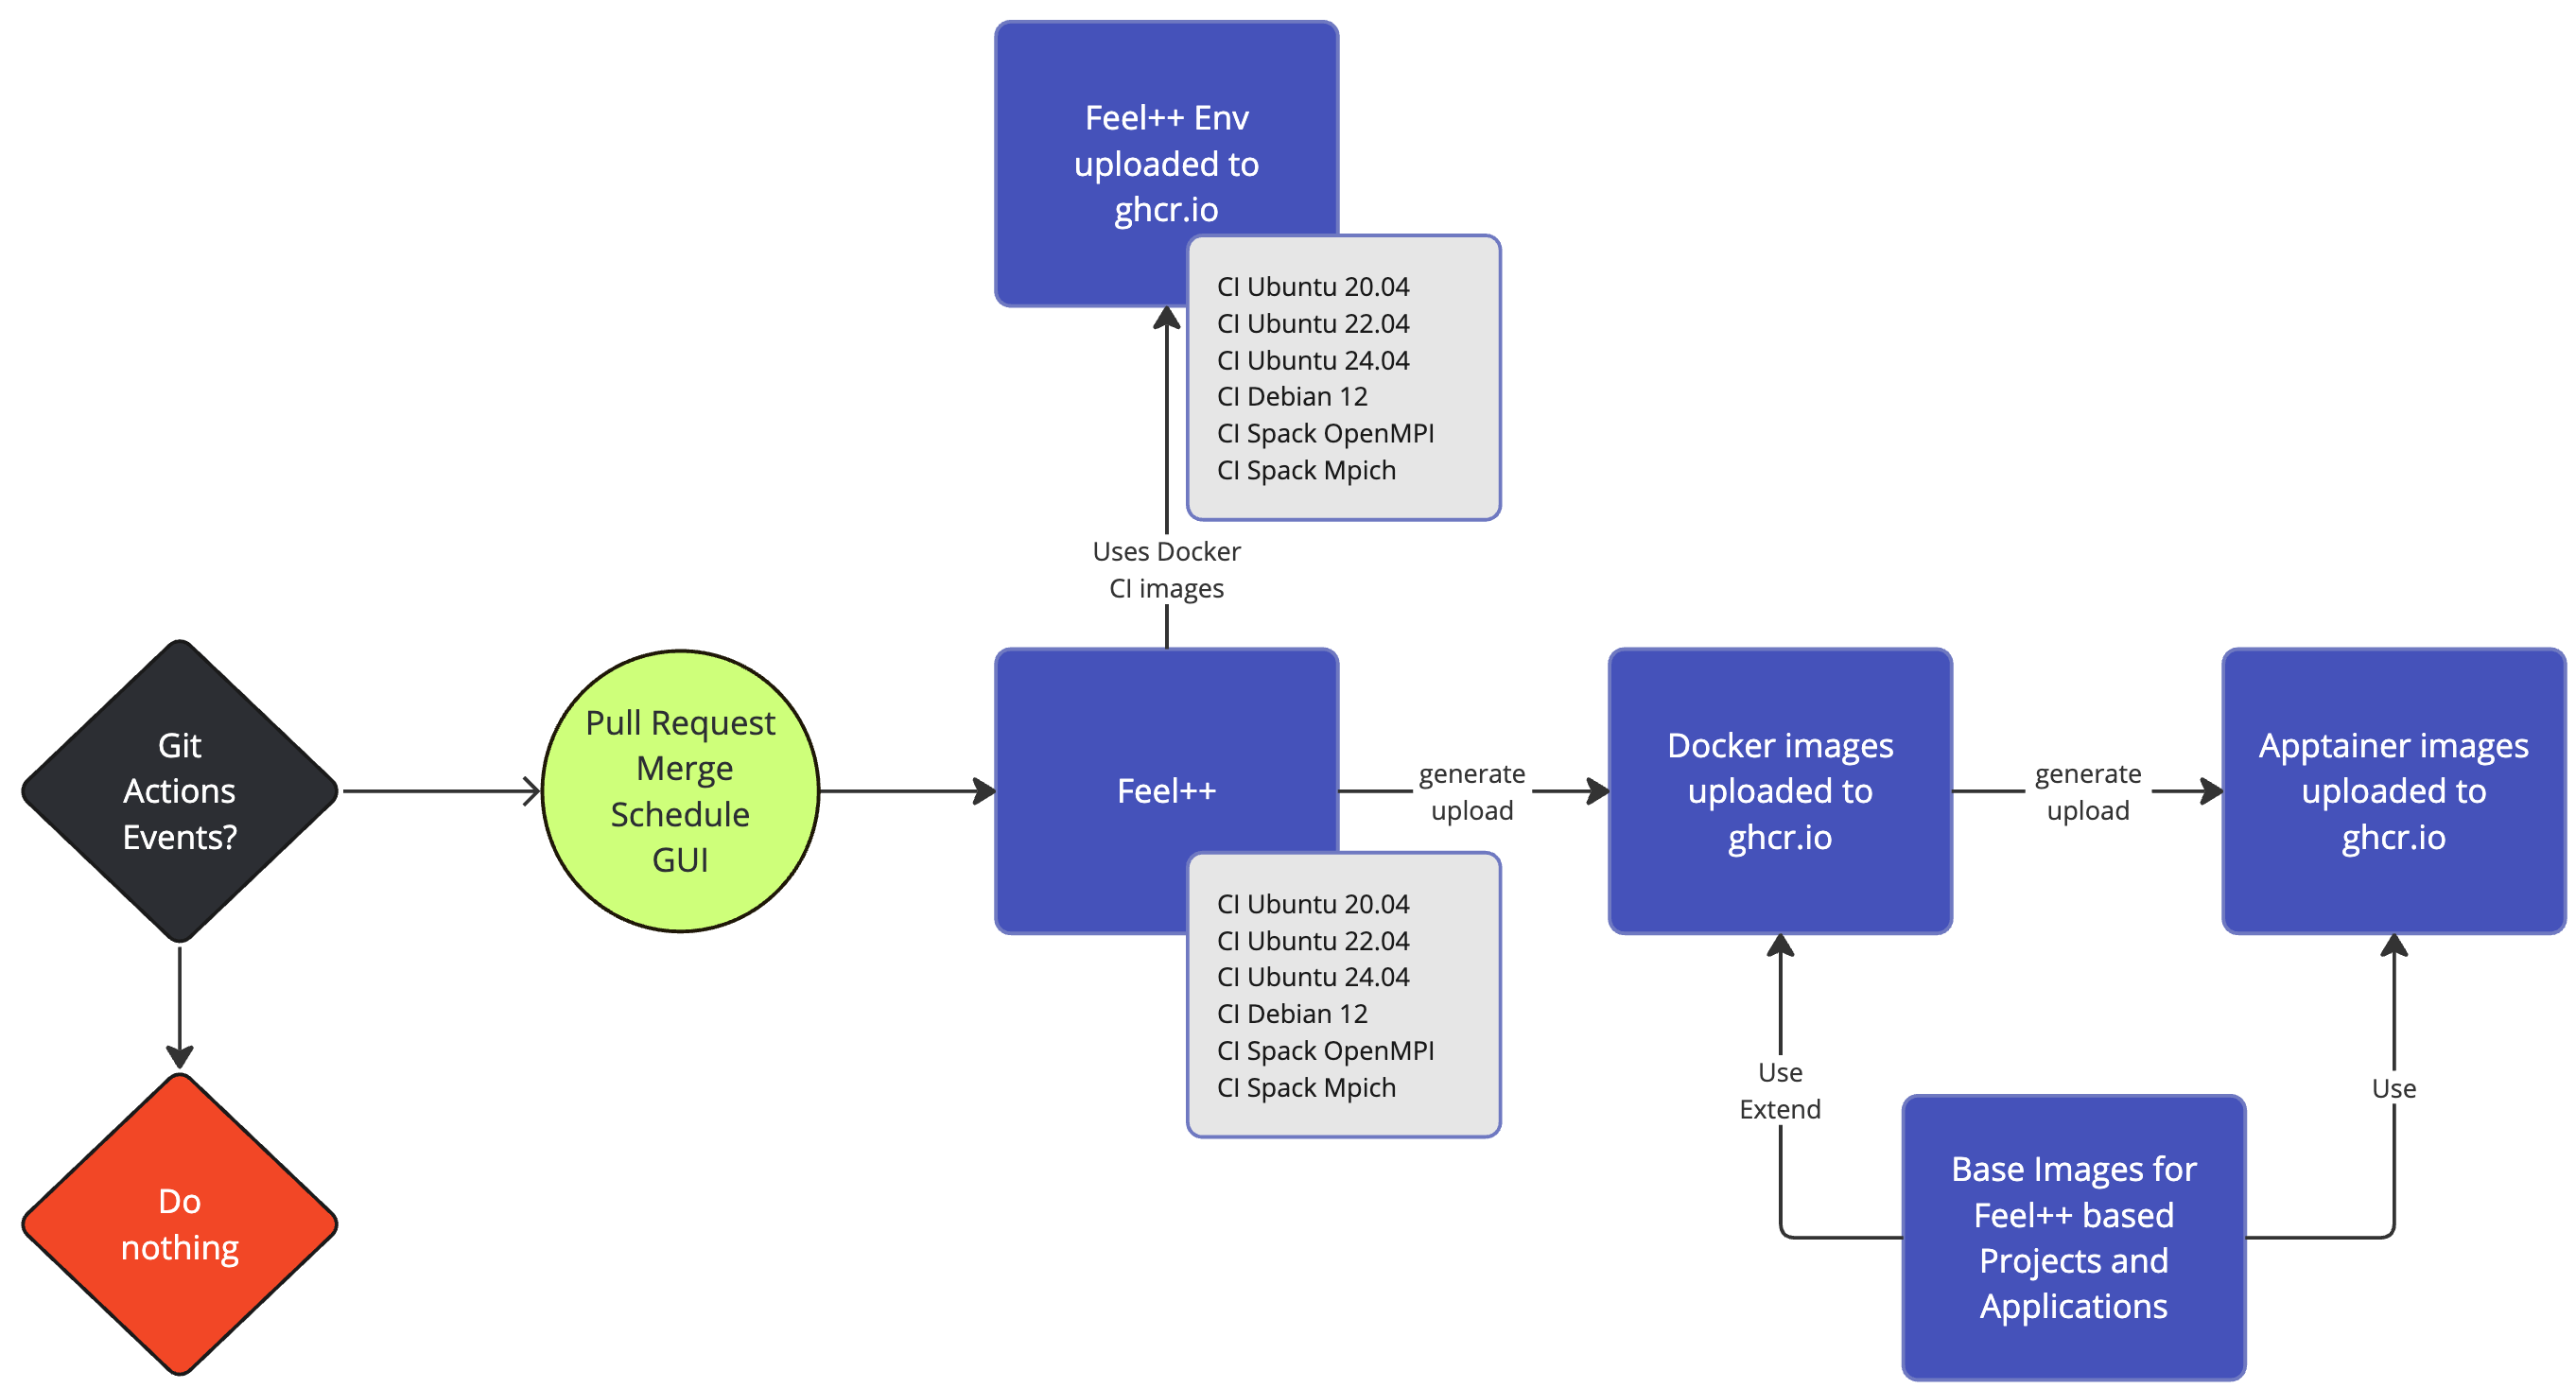
\includegraphics[width=0.8\textwidth]{graphics/feelpp/feelpp-ci-workflow.png}
        \caption{\Feelpp Continuous Integration Workflow using GitHub Actions}
        \label{fig:feelpp-ci}
    \end{figure}

    The~\Cref{fig:feelpp-cb} shows the \Feelpp Continuous Benchmarking Workflow using GitHub Actions and Reframe which is quite close to the methodology described in~\Cref{sec:methodology-regression-reframe}.
    \begin{figure}
        \centering
        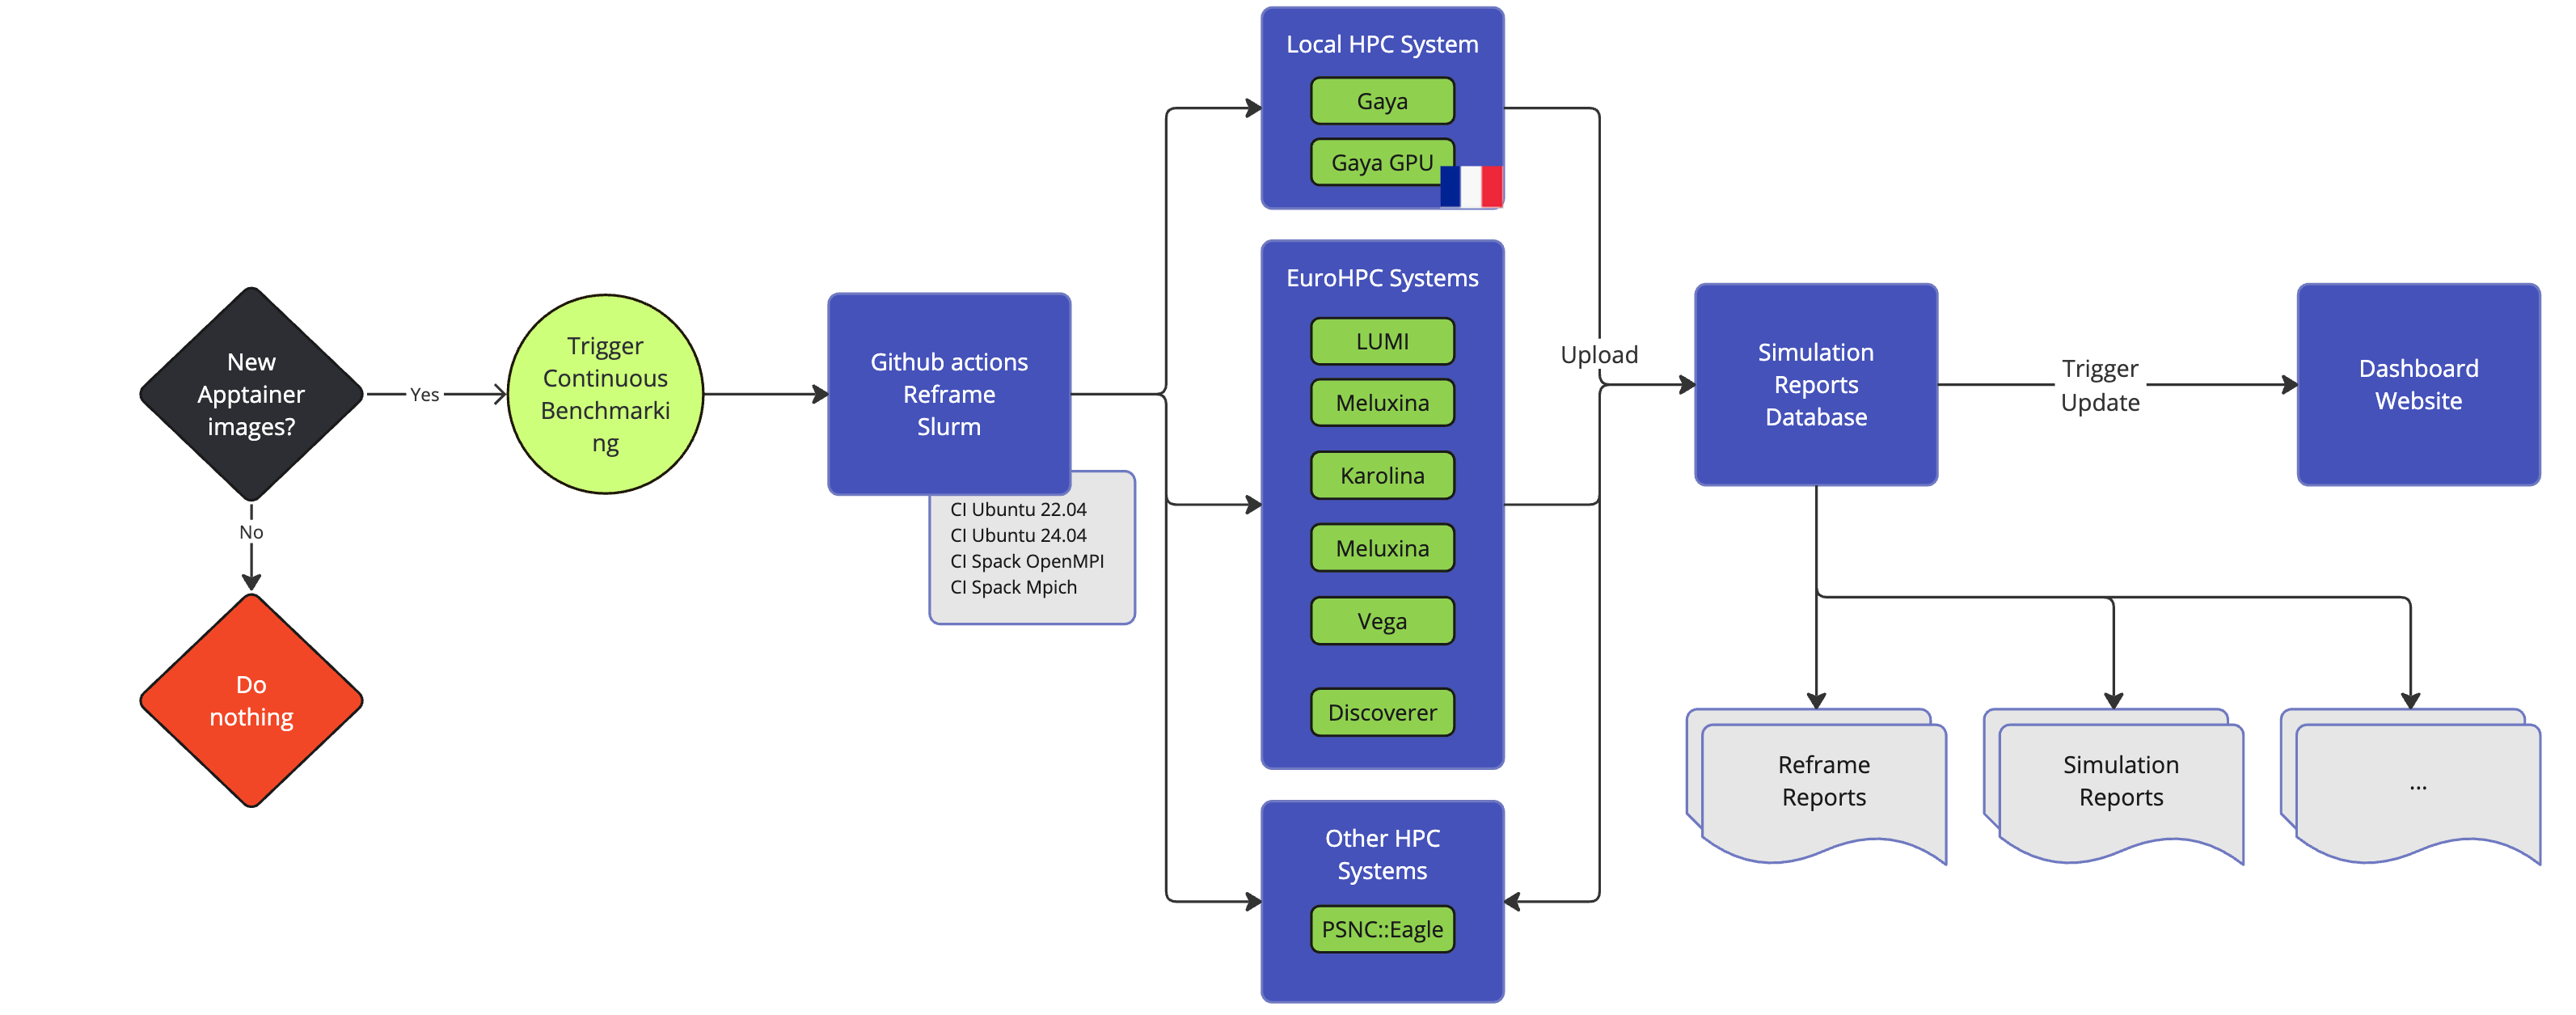
\includegraphics[width=0.8\textwidth]{graphics/feelpp/feelpp-cb-workflow.png}
        \caption{\Feelpp Continuous Benchmarking Workflow using GitHub Actions and Reframe}
        \label{fig:feelpp-cb}
    \end{figure}

\subsection{Mathematics}
\label{sec:Feelpp:mathematics}
\Feelpp is based on the \ac{FEM}, which is used for solving partial differential equations (PDEs) in complex geometries.
It leverages advanced numerical techniques to ensure accuracy and scalability, including adaptive mesh refinement, domain decomposition, and error estimation.

The~\Cref{fig:Feelpp:components} shows the main components of \Feelpp, including the finite element method, mesh generation, solvers but also the components that will be tested in the benchmarks of this deliverable.

\begin{figure}
        \centering
        %!TEX root = ../exa-ma-d7.1.tex

\definecolor{mybluei}{RGB}{70, 82, 186}
\definecolor{myblueii}{RGB}{73,121,193}
\definecolor{mygreen}{RGB}{142, 209, 79}
\definecolor{mypink}{RGB}{255,248,241}

\newcommand\widernode[5][widebox]{
  \node[
    #1,
    fit={(#2) (#3)},
    label=center:{\sffamily\bfseries\color{white}#4}] (#5) {};
}

\begin{tikzpicture}[node distance=3pt,outer sep=0pt,
boxstyle/.style={
  draw=white,
  fill=#1,
  rounded corners,
  font={\sffamily\bfseries\color{white}},
  align=center,
  minimum height=30pt
},
box/.style={
  boxstyle=#1,
  text width=2.5cm},
box/.default=mybluei,
title/.style={font={\sffamily\bfseries\color{white}}},
widebox/.style={draw=white,inner sep=0pt, rounded corners,fill=#1},
widebox/.default=mybluei,
mylabel/.style={font={\sffamily\bfseries\color{white}}},
]

\matrix (stack) [boxstyle=mybluei!40, draw=black,%
        column sep=3pt, row sep=3pt, inner sep=4mm,%
      matrix of nodes,%
        nodes={box, outer sep=0pt, anchor=center, inner sep=3pt},%
        nodes in empty cells,
      %row 1/.style={nodes={fill=none,draw=none,minimum height=3mm}},
]
{
  & & & & \\
& & & & \\  
& & & & \\
& & & & \\
 &  &  &  & Models Description\\
Space Cartesian Products &  & PDE based Preconditioners & Ray-Tracing (BVH) & Level-Set (FastMarching) \\
 & & & &  Forms\\
Finite Elements & Geometric Mapping & & & Export/Import\\
 Timings & & &  &  Quadratures \\
& & & & \\};
\widernode[widebox=mygreen]{stack-1-1}{stack-1-5}{\begin{tabular}{c}Advanced Methods and Analysis:\\ Inverse Problems, Data Assimilation, UQ, ML\ldots \end{tabular}}{Analysis}
\widernode[widebox=mygreen]{stack-2-1}{stack-2-5}{\begin{tabular}{c}Python bindings:\\ Core, \Feelpp Libs, Toolboxes, MOR\end{tabular}}{Python}
\widernode[widebox=mygreen]{stack-3-1}{stack-3-5}{\begin{tabular}{c}ROM: \\RB(Greedy,POD,Error Bounds, SCM/Min-$\theta$, NL-C), (D,G)EIM, PBDW, NIRB\end{tabular}}{RB}
\widernode[widebox=mygreen]{stack-4-1}{stack-4-5}{\begin{tabular}{c}Toolboxes: \\ ALE, CFPDEs, CFD, CSM, Heat, HeatFluid, FSI, ThermoElectric, Maxwell\end{tabular}}{Toolboxes}
\widernode{stack-5-3}{stack-5-4}{Models Description: JSON...}{model}
\widernode{stack-5-1}{stack-5-2}{DSEL for Galerkin Methods}{dsel}
\widernode{stack-6-1}{stack-6-2}{\begin{tabular}{c}Cartesian Products:\\ Spaces, Functions and Forms\end{tabular}}{prod}
\widernode{stack-7-3}{stack-7-4}{Interpolation}{interp}
\widernode{stack-7-1}{stack-7-2}{Function Spaces}{fespace}
\widernode{stack-8-3}{stack-8-3}{Mesh}{Mesh}
\widernode{stack-8-4}{stack-8-4}{Time Discr.}{TimeD}
%\widernode{stack-5-4}{stack-5-5}{Export/Import}{ExImp}
\widernode{stack-9-2}{stack-9-4}{Linear Algebra:
  preconditioner framework, ...}{Alg}
\widernode[widebox=mygreen]{stack-10-1}{stack-10-5}{Core: Environment,
  Logging, Monitoring, Events, Communicators ...}{Core}

\node [fit={(stack.north west)(stack.north
  east)},boxstyle=mybluei!60,draw=black,inner sep=0pt,above=3pt of
stack.north,anchor=south,label={[mylabel]center: Applications: Ktirio Urban Building, Eye2Brain, Swimmer, HifiMagnet}] (AnalysisTools) {};
\node [fit={(stack.south west)(stack.south
  east)},boxstyle=mybluei!60,draw=black,inner sep=0pt,below=3pt of
stack.south,anchor=north,label={[mylabel]center:  Python3, Gmsh, MMG, CGAL, OpenTURNS,  OpenModelica, Salome}] (DepsTools) {};
  \node [fit={(DepsTools.south west)(DepsTools.south
  east)},boxstyle=mybluei!60,draw=black,inner sep=0pt,below=3pt of
DepsTools.south,anchor=north,label={[mylabel]center: C++17, MPI, Boost,
  Google::Glog, MongoDB, Eigen3, PETSc/SLEPc}] (Deps) {};

\end{tikzpicture}

        \caption{Main dependencies of \Feelpp(bottom rows), its main Components as well as the flagship applications (top row).}
        \label{fig:Feelpp:components}
\end{figure}



\subsection{Relevant Publications}
\label{sec:Feelpp:publications}
Relevant publications include:

\begin{description}
        \item[\fullcite{prudhomme_feel_2012}] presents a detailed exploration of \Feelpp's design, focusing on its embedded variational language as a \ac{DSEL} and abstraction mechanisms that simplify the implementation of complex numerical methods. The framework is demonstrated with examples involving non-overlapping domain decomposition techniques and fictitious domain methods.
        \item[\fullcite{prudhomme_feelppfeelpp_2024}] is the last preview of the \Feelpp software. The documentation is available online at \url{https://docs.feelpp.org};
        \item[\fullcite{van_landeghem_mathematical_2024}] The paper \emph{Mathematical and computational framework for moving and colliding rigid bodies in a Newtonian fluid} (2024) presents a mathematical model and computational strategy to simulate the dynamics of moving and colliding rigid bodies within a Newtonian fluid. This work focuses on accurately modeling fluid-structure interactions as a step towards simulating micro-swimmers.
        \item[\fullcite{saigre_model_2024}] The paper \emph{Model Order Reduction and Sensitivity Analysis for Complex Heat Transfer Simulations Inside the Human Eyeball}, presents advanced computational methods to simulate heat transfer processes within the human eye. The authors use reduced-order modeling to improve the efficiency and accuracy of these simulations, contributing to better insights in biomedical engineering through advanced analysis and in particular sensitivity analysis.;
        \item[\fullcite{prudhomme_ktirio_2024}] The paper \emph{Ktirio Urban Building: A Computational Framework for City Energy Simulations Enhanced by CI/CD Innovations on EuroHPC Systems} (2024) presents a high-performance computational framework designed to support the European Union's Horizon 2050 initiative by improving energy consumption in buildings at city scale and beyond. The framework, known as Ktirio Urban Building (KUB), leverages Continuous Integration/Continuous Deployment (CI/CD) innovations to streamline large-scale city energy simulations on EuroHPC JU supercomputers.
        \item[\fullcite{saigre_coupled_2024_abstract}] The paper \emph{A coupled fluid-dynamics-heat transfer model for 3D simulations of the aqueous humor flow in the human eye} presents a coupled fluid-dynamics-heat transfer model to simulate the flow of aqueous humor in the human eye, providing insights into the impact of the postural orientation of the patient on the fluid dynamics and heat transfer processes within the eye. An full-length paper of this extended abstract is in preparation \cite{saigre_coupled_2024_paper}.
        \item[\fullcite{palazzolo2023shape}] The master thesis \emph{Shape Optimization for Rigid Objects in a Stokes Flow} (2023) presents a comprehensive study of shape optimization for rigid objects within a Stokes flow. The research focuses on determining the optimal shapes of 2D and 3D objects using iterative methods, including gradient descent and null-space techniques. The implementation of this work is publicly available at \url{https://feelpp.github.io/feelpp-shapo/shapo/index.html}.
\end{description}

\subsection{Acknowledgements}
\label{sec::Feelpp:acknowledgements}
The software has been developed with the support of the following funding agencies and institutions through various research projects:
\begin{itemize}
   \item Université de Strasbourg
   \item Cemosis
   \item CNRS
   \item ANR
   \item Région Grand Est
   \item AMIES
   \item European Commission
   \item EuroHPC JU
\end{itemize}

\section{Software: FreeFem++}
\label{sec:FreeFem++:software}



\begin{itemize}
    \item \textbf{Contact Email(s):} frederic.hecht@sorbonne-universite.fr, pierre.jolivet@sorbonne-universite.fr
    \item \textbf{Supported Architecture(s):} CPU
    \item \textbf{Repository Link:} \href{https://github.com/FreeFem/FreeFem-sources}{https://github.com/FreeFem/FreeFem-sources}
\end{itemize}

\subsection{Software summary}
\label{sec:FreeFem++:summary}
Detailed overview not available.



\subsection{Purpose}
\label{sec:FreeFem++:purpose}
Purpose not available.



\subsection{Mathematics}
\label{sec:FreeFem++:mathematics}
Mathematics not available.


\subsection{Relevant Publications}
\label{sec:FreeFem++:publications}

\subsection{Acknowledgements}
\label{sec::FreeFem++:acknowledgements}

Acknowledgements not available.



\section{Software: Hawen}
\label{sec:Hawen:software}



\begin{table}[h!]
    \centering
    { \setlength{\parindent}{0pt}
    \def\arraystretch{1.25}
    \arrayrulecolor{numpexgray}
    {\fontsize{9}{11}\selectfont
    \begin{tabular}{!{\color{numpexgray}\vrule}p{.4\textwidth}!{\color{numpexgray}\vrule}p{.6\textwidth}!{\color{numpexgray}\vrule}}
        \rowcolor{numpexgray}{\rule{0pt}{2.5ex}\color{white}\bf Field} & {\rule{0pt}{2.5ex}\color{white}\bf Details} \\
        \rowcolor{white}\textbf{Consortium} & \begin{tabular}{l}
Inria\\
\end{tabular} \\
        \rowcolor{numpexlightergray}\textbf{Exa-MA Partners} & \begin{tabular}{l}
Inria BXSO\\
\end{tabular} \\
        \rowcolor{white}\textbf{Contact Emails} & \begin{tabular}{l}
florian.faucher@inria.fr\\
\end{tabular} \\
        \rowcolor{numpexlightergray}\textbf{Supported Architectures} & \begin{tabular}{l}
CPU Only\\
\end{tabular} \\
        \rowcolor{white}\textbf{Repository} & \href{https://gitlab.com/ffaucher/hawen}{https://gitlab.com/ffaucher/hawen} \\
        \rowcolor{numpexlightergray}\textbf{License} & \begin{tabular}{l}
OSS:: GPL v*\\
\end{tabular} \\
        \rowcolor{white}\textbf{Bottlenecks roadmap} & \begin{tabular}{l}
B10 - Scientific Productivity\\
B11 - Reproducibility and Replicability of Computation\\
B6 - Data Management\\
B7 - Exascale Algorithms\\
\end{tabular} \\
        \bottomrule
    \end{tabular}
    }}
    \caption{Hawen Information}
\end{table}

% ---------------------------------------------
\newcommand{\hawen}{\textsc{Hawen}}
\subsection{Software summary}
\label{sec:Hawen:summary}
% ---------------------------------------------

Software \hawen~(\url{https://ffaucher.gitlab.io/hawen-website/})
considers the time-harmonic modeling of mechanical waves, and the 
associated quantitative inverse wave problems.
The code uses the Hybridizable Discontinuous Galerkin method (HDG) 
for the discretization. 
It relies on nonlinear iterative minimization algorithm to solve 
the quantitative inverse wave problem.
The code is written in \texttt{Fortran90} and uses \texttt{mpi}
and \texttt{OpenMP} parallelism.



\subsection{Purpose}
\label{sec:Hawen:purpose}

\hawen~solves large-scale inverse wave problems in the frequency domain, 
with an emphasis on applications in the context of Earth's imaging and helioseismology.


\subsection{Programming and Computational Environment}
\label{sec::Hawen:environment_capabilities}


The following table~\ref{table:hawen-environment} summarizes these aspects for \hawen, providing a  view of its programming and computational capabilities.

\begin{table}[h!]
    \centering
    {
    \setlength{\parindent}{0pt}
    \def\arraystretch{1.25}
    \arrayrulecolor{numpexgray}
    {\fontsize{9}{11}\selectfont
    \begin{tabular}{lp{.3\textwidth}p{.5\textwidth}}
        \rowcolor{numpexgray}{\rule{0pt}{2.5ex}\color{white}\bf Category}  & {\rule{0pt}{2.5ex}\color{white}\bf Details} & {\rule{0pt}{2.5ex}\color{white}\bf Description}\\
        \rowcolor{white}Languages  & \begin{tabular}{l}
Fortran\\
\end{tabular} & Programming languages and language standards supported by the software \\
        \rowcolor{numpexlightergray}Parallelism  & \begin{tabular}{l}
MPI\\
Multithread\\
\end{tabular} & Parallel computing methods and frameworks utilized by the software.\\
        \rowcolor{white}Data Formats  & \begin{tabular}{l}
Gmsh and associated formats\\
VTK\\
in-house binary format\\
\end{tabular} & Data formats that the software can handle or produce.
Gmsh format can be used for input mesh. 
VTK or binary format can be used to save the results such as the 
wave propagation solutions.
\\
        \rowcolor{numpexlightergray}Resilience  & \begin{tabular}{l}
None\\
\end{tabular} & Fault tolerance and recovery mechanisms employed by the software.\\
        \rowcolor{white}DevOps & \begin{tabular}{l}
None\\
\end{tabular} & Outlines the development and operational practices including continuous integration, containerization, and testing methodologies.  \\
        \rowcolor{numpexlightergray}Packaging  & \begin{tabular}{l}
None\\
\end{tabular} & Software packaging and distribution.\\
        \rowcolor{white}Testing  & \begin{tabular}{l}
Analytic solutions\\
\end{tabular} & Testing methodologies employed to ensure software quality and correctness:
Analytic solutions for the propagation of acoustic and elastic waves, respectively 
\eqref{eq:hawen:viscoacoustic} and \eqref{eq:hawen:viscoelastic} exist and are compared 
with the numerical resolutions. For instance we refer to \cite{Pham2024stabilization} for 
the validation of the linear elasticity propagator.
\\
        \rowcolor{numpexlightergray}Containerization  & \begin{tabular}{l}
None\\
\end{tabular} & Container technologies used to package and deploy the software.\\
        \rowcolor{white}Interfaces  & \begin{tabular}{l}
MUMPS\\ 
Metis\\ 
ARPACK (optional)\\
PARPACK (optional)\\
\end{tabular} & List of software Hawen has interfaces with.
        MUMPS is used to solve the linear system resulting from 
        the numerical discretization. Metis is used to partition
        the mesh. ARPACK and PARPACK are optional dependencies 
        used for eigenproblems.\\
        \bottomrule
    \end{tabular}
    }}
    \caption{Hawen programming and computational environment}
    \label{table:hawen-environment}
\end{table}



\subsection{Mathematics}
\label{sec:Hawen:mathematics}

\paragraph{Forward problem} \hawen~allows for the modeling of time-harmonic
mechanical waves for different types of media. 
By using the HDG method for the discretization, we work with first-order systems.
In the case of visco-acoustics wave propagation, the forward problem consists in
finding the scalar pressure field $p$ and vector velocity field $\boldsymbol{v}$ 
such that
\begin{subequations}\label{eq:hawen:viscoacoustic}
\begin{empheq}[left={\empheqlbrace}]{align}
 &-\mathrm{i}\omega \rho \boldsymbol{v} \,+\, \nabla p \,=\, 0 \,, \\
 &-\dfrac{\mathrm{i}\omega}{\kappa} p \,+\, \nabla\cdot\boldsymbol{v} \,=\, f \,,
\end{empheq}\end{subequations}
where $\omega$ is the angular frequency, and the medium is characterized
by the density $\rho$ and the bulk modulus $\kappa$. The source term is 
$f$. 
We further refer to \cite{Faucher2020adjoint,Faucher2023viscoacoustic}
for more details.
The code allows for different types of boundary conditions, such as 
imposing the Dirichlet trace, Neumann trace, or a Robin-type condition
(e.g., for radiation condition).


In the case of linear visco-elastic wave propagation, the forward problem consists in
finding the displacement field $\boldsymbol{u}$ and stress tensor $\boldsymbol{\sigma}$ 
solutions to, cf., e.g., \cite{Pham2024stabilization},
\begin{subequations}\label{eq:hawen:viscoelastic}
\begin{empheq}[left={\empheqlbrace}]{align}
 &-\omega^2\rho\boldsymbol{u} \,-\, \nabla\cdot\boldsymbol{\sigma}\,=\,\boldsymbol{f} \,, \\
 & \boldsymbol{\sigma} \,=\, \boldsymbol{C} \, \big(\nabla\boldsymbol{u} \,+\, (\nabla\boldsymbol{u})^t\big) \,.
\end{empheq}\end{subequations}
Here, the medium is characterized by the density 
$\rho$ and the stiffness tensor $\boldsymbol{C}$,
we refer to \cite{Pham2024stabilization}
for more details related to HDG implementation.

In the context of helioseismology, we consider the scalar-wave propagation 
which comes from simplification of the Galbrun's equation, 
cf.~\cite{Pham2020Siam,Pham2024assembling}, in three dimensions, the 
simplest form corresponds to finding $u$ solution to: 
\begin{equation} \label{eq:hawen:helio-scalar}
  \Big( \,-\nabla \,-\,\dfrac{\omega^2}{c^2} \,+\, q \Big) \, u \,=\, f\,,
\end{equation}
with potential $q$, sound-speed $c$ and source term $f$. 
In addition, \hawen~solves the problem under the assumption of 
spherical symmetry and we refer to \cite{Pham2020Siam} for more 
details. 
Several choices of radiation boundary conditions have been 
implemented and tested, cf.~\cite{Pham2019radiationBC,Pham2020Siam}.
Recently, more complete equations to model the Sun have 
been implemented in \hawen, see \cite{Pham2024assembling}.

\paragraph{Inversion} 
\hawen~solves the inverse problems for the reconstruction of the 
model parameters from the measurements of waves. For instance, 
considering the acoustic wave equation \eqref{eq:hawen:viscoacoustic},
it consists in finding the density $\rho$ and bulk modulus $\kappa$
from the observations of the pressure $p$ and/or velocity field $\boldsymbol{v}$
at a discrete set of positions.
\hawen~employs a nonlinear iterative minimization algorithm for the 
reconstruction of the properties, as illustrated in 
\cite{Hawen2021,Faucher2019FRgWIGeo,Faucher2020DAS,Faucher2023viscoacoustic}.
This approach is typically referred to as the \emph{Full Waveform Inversion}
in the context of seismic imaging, cf. \cite{Virieux2009} for a review.


\subsection{Relevant Publications}
\label{sec:Hawen:publications}

Here is a list of relevant publications related to the software:
\begin{itemize}
\item \cite{Hawen2021}: Reference of the software in the journal of open-source software;
\item \cite{Faucher2020adjoint}:
      Mathematical details of the adjoint-state method in the framework 
      of Hybridizable Discontinuous Galerkin discretization method.
      It provides the computational steps for the implementation of the 
      inverse problem.
\item \cite{Pham2024stabilization}: Details of the numerical implementation 
      of the HDG method for anisotropic elasticity.
\item \cite{Faucher2019FRgWIGeo,Faucher2020DAS}: 
      Use of the software in the context of seismic imaging.
\item \cite{Pham2020Siam,Pham2024assembling}:
      Use of the software in the context of helioseismology.
\item \cite{Faucher2023viscoacoustic}: 
      Use of the software in the context of viscoacoustics ultrasound imaging.
\item \cite{Liu2024,Benitez2024}: 
      Use of the software in the context of data science and
      for benchmarks.
\end{itemize}


\subsection{Acknowledgements}
\label{sec::Hawen:acknowledgements}

The software has been developed with the support of the following funding agencies and institutions: 

\begin{itemize}
  \item Since 2021, F. Faucher is part of the team Makutu of INRIA Bordeaux, at the 
                    University of Pau and Pays de l'Adour.
  \item 2024--2029, F. Faucher acknowledges support of the European Research Council 
                    with ERC-StG Project INCORWAVE -- grant 101116288.
  \item 2019--2021, F. Faucher acknowledges funding by the Austrian Science Fund (FWF) 
        under the Lise Meitner grant allocation M2791-N.
\end{itemize}



\section{Software: HPDDM}
\label{sec:HPDDM:software}



\begin{table}[h!]
    \centering
    { \setlength{\parindent}{0pt}
    \def\arraystretch{1.25}
    \arrayrulecolor{numpexgray}
    {\fontsize{9}{11}\selectfont
    \begin{tabular}{!{\color{numpexgray}\vrule}p{.4\textwidth}!{\color{numpexgray}\vrule}p{.6\textwidth}!{\color{numpexgray}\vrule}}
        \rowcolor{numpexgray}{\rule{0pt}{2.5ex}\color{white}\bf Field} & {\rule{0pt}{2.5ex}\color{white}\bf Details} \\
        \rowcolor{white}\textbf{Consortium} & \begin{tabular}{l}
None\\
\end{tabular} \\
        \rowcolor{numpexlightergray}\textbf{Exa-MA Partners} & \begin{tabular}{l}
Inria PARIS\\
Sorbonne U\\
\end{tabular} \\
        \rowcolor{white}\textbf{Contact Emails} & \begin{tabular}{l}
pierre@joliv.et\\
\end{tabular} \\
        \rowcolor{numpexlightergray}\textbf{Supported Architectures} & \begin{tabular}{l}
CPU or GPU\\
\end{tabular} \\
        \rowcolor{white}\textbf{Repository} & \href{https://github.com/hpdomain decomposition methods/hpdomain decomposition methods}{https://github.com/hpdomain decomposition methods/hpdomain decomposition methods} \\
        \rowcolor{numpexlightergray}\textbf{License} & \begin{tabular}{l}
OSS:: LGPL v*\\
\end{tabular} \\
        \rowcolor{white}\textbf{Bottlenecks roadmap} & \begin{tabular}{l}
B10 - Scientific Productivity\\
B11 - Reproducibility and Replicability of Computation\\
B6 - Data Management\\
B7 - Exascale Algorithms\\
\end{tabular} \\
        \bottomrule
    \end{tabular}
    }}
    \caption{HPDDM Information}
\end{table}

\subsection{Software summary}
\label{sec:HPDDM:summary}
Detailed overview not available.



\subsection{Purpose}
\label{sec:HPDDM:purpose}
Purpose not available.

\subsection{Programming and Computational Environment}
\label{sec::HPDDM:environment_capabilities}


The following table summarizes these aspects for HPDDM, providing a  view of its programming and computational capabilities.

\begin{table}[h!]
    \centering
    {
    \setlength{\parindent}{0pt}
    \def\arraystretch{1.25}
    \arrayrulecolor{numpexgray}
    {\fontsize{9}{11}\selectfont
    \begin{tabular}{lp{.3\textwidth}p{.5\textwidth}}
        \rowcolor{numpexgray}{\rule{0pt}{2.5ex}\color{white}\bf Category}  & {\rule{0pt}{2.5ex}\color{white}\bf Details} & {\rule{0pt}{2.5ex}\color{white}\bf Description}\\
        \rowcolor{white}Languages  & \begin{tabular}{l}
C\\
C++\\
Fortran\\
Python\\
\end{tabular} & Programming languages and language standards supported by the software \\
        \rowcolor{numpexlightergray}Parallelism  & \begin{tabular}{l}
GPU\\
MPI\\
Multithread\\
\end{tabular} & Parallel computing methods and frameworks utilized by the software.\\
        \rowcolor{white}Data Formats  & \begin{tabular}{l}
in-house format\\
\end{tabular} & Data formats that the software can handle or produce.\\
        \rowcolor{numpexlightergray}Resilience  & \begin{tabular}{l}
None\\
\end{tabular} & Fault tolerance and recovery mechanisms employed by the software.\\
        \rowcolor{white}DevOps & \begin{tabular}{l}
Continuous Integration\\
\end{tabular} & Outlines the development and operational practices including continuous integration, containerization, and testing methodologies.  \\
        \rowcolor{numpexlightergray}Packaging  & \begin{tabular}{l}
None\\
\end{tabular} & Software packaging and distribution.\\
        \rowcolor{white}Testing  & \begin{tabular}{l}
Unit\\
Verification\\
\end{tabular} & Testing methodologies employed to ensure software quality and correctness.\\
        \rowcolor{numpexlightergray}Containerization  & \begin{tabular}{l}
None\\
\end{tabular} & Container technologies used to package and deploy the software.\\
        \rowcolor{white}Interfaces  & \begin{tabular}{l}
Feel++\\
Freefem++\\
MUMPS\\
PETSc\\
PaStiX\\
\end{tabular} & List of software HPDDM has interfaces with.\\
        \bottomrule
    \end{tabular}
    }}
    \caption{HPDDM programming and computational environment}
\end{table}



\subsection{Mathematics}
\label{sec:HPDDM:mathematics}
Mathematics not available.

In this section, provide a summary the mathematics used in the software.


\subsection{Relevant Publications}
\label{sec:HPDDM:publications}

Here is a list of relevant publications related to the software:


\subsection{Acknowledgements}
\label{sec::HPDDM:acknowledgements}

The software has been developed with the support of the following funding agencies and institutions: 




Acknowledgements not available.



%%\section{Software: MaHyCo}
\label{sec:MaHyCo:software}



\begin{table}[h!]
    \centering
    { \setlength{\parindent}{0pt}
    \def\arraystretch{1.25}
    \arrayrulecolor{numpexgray}
    {\fontsize{9}{11}\selectfont
    \begin{tabular}{!{\color{numpexgray}\vrule}p{.4\textwidth}!{\color{numpexgray}\vrule}p{.6\textwidth}!{\color{numpexgray}\vrule}}
        \rowcolor{numpexgray}{\rule{0pt}{2.5ex}\color{white}\bf Field} & {\rule{0pt}{2.5ex}\color{white}\bf Details} \\
        \rowcolor{white}\textbf{Consortium} & \begin{tabular}{l}
CEA\\
\end{tabular} \\
        \rowcolor{numpexlightergray}\textbf{Exa-MA Partners} & \begin{tabular}{l}
CEA\\
\end{tabular} \\
        \rowcolor{white}\textbf{Contact Emails} & \begin{tabular}{l}
jean-philippe.perlat@cea.fr\\
\end{tabular} \\
        \rowcolor{numpexlightergray}\textbf{Supported Architectures} & \begin{tabular}{l}
CPU or GPU\\
\end{tabular} \\
        \rowcolor{white}\textbf{Repository} & \href{https://github.com/cea-hpc/MaHyCo}{https://github.com/cea-hpc/MaHyCo} \\
        \rowcolor{numpexlightergray}\textbf{License} & \begin{tabular}{l}
OSS: apache-2\\
\end{tabular} \\
        \rowcolor{white}\textbf{Bottlenecks roadmap} & \begin{tabular}{l}
B10 - Scientific Productivity\\
B11 - Reproducibility and Replicability of Computation\\
B6 - Data Management\\
B7 - Exascale Algorithms\\
\end{tabular} \\
        \bottomrule
    \end{tabular}
    }}
    \caption{MaHyCo Information}
\end{table}

\subsection{Software summary}
\label{sec:MaHyCo:summary}
Detailed overview not available.



\subsection{Purpose}
\label{sec:MaHyCo:purpose}
Purpose not available.

\subsection{Programming and Computational Environment}
\label{sec::MaHyCo:environment_capabilities}


The following table summarizes these aspects for MaHyCo, providing a  view of its programming and computational capabilities.

\begin{table}[h!]
    \centering
    {
    \setlength{\parindent}{0pt}
    \def\arraystretch{1.25}
    \arrayrulecolor{numpexgray}
    {\fontsize{9}{11}\selectfont
    \begin{tabular}{lp{.3\textwidth}p{.5\textwidth}}
        \rowcolor{numpexgray}{\rule{0pt}{2.5ex}\color{white}\bf Category}  & {\rule{0pt}{2.5ex}\color{white}\bf Details} & {\rule{0pt}{2.5ex}\color{white}\bf Description}\\
        \rowcolor{white}Languages  & \begin{tabular}{l}
C++\\
\end{tabular} & Programming languages and language standards supported by the software \\
        \rowcolor{numpexlightergray}Parallelism  & \begin{tabular}{l}
GPU\\
MPI\\
\end{tabular} & Parallel computing methods and frameworks utilized by the software.\\
        \rowcolor{white}Data Formats  & \begin{tabular}{l}
XML\\
\end{tabular} & Data formats that the software can handle or produce.\\
        \rowcolor{numpexlightergray}Resilience  & \begin{tabular}{l}
Checkpoint restart\\
\end{tabular} & Fault tolerance and recovery mechanisms employed by the software.\\
        \rowcolor{white}DevOps & \begin{tabular}{l}
Continuous Integration\\
\end{tabular} & Outlines the development and operational practices including continuous integration, containerization, and testing methodologies.  \\
        \rowcolor{numpexlightergray}Packaging  & \begin{tabular}{l}
None\\
\end{tabular} & Software packaging and distribution.\\
        \rowcolor{white}Testing  & \begin{tabular}{l}
None\\
\end{tabular} & Testing methodologies employed to ensure software quality and correctness.\\
        \rowcolor{numpexlightergray}Containerization  & \begin{tabular}{l}
None\\
\end{tabular} & Container technologies used to package and deploy the software.\\
        \rowcolor{white}Interfaces  & \begin{tabular}{l}
Arcane Framework\\
\end{tabular} & List of software MaHyCo has interfaces with.\\
        \bottomrule
    \end{tabular}
    }}
    \caption{MaHyCo programming and computational environment}
\end{table}



\subsection{Mathematics}
\label{sec:MaHyCo:mathematics}
Mathematics not available.

In this section, provide a summary the mathematics used in the software.


\subsection{Relevant Publications}
\label{sec:MaHyCo:publications}

Here is a list of relevant publications related to the software:


\subsection{Acknowledgements}
\label{sec::MaHyCo:acknowledgements}

The software has been developed with the support of the following funding agencies and institutions: 




Acknowledgements not available.



\section{Software: MANTA}
\label{sec:MANTA:software}



\begin{table}[h!]
    \centering
    { \setlength{\parindent}{0pt}
    \def\arraystretch{1.25}
    \arrayrulecolor{numpexgray}
    {\fontsize{9}{11}\selectfont
    \begin{tabular}{!{\color{numpexgray}\vrule}p{.4\textwidth}!{\color{numpexgray}\vrule}p{.6\textwidth}!{\color{numpexgray}\vrule}}
        \rowcolor{numpexgray}{\rule{0pt}{2.5ex}\color{white}\bf Field} & {\rule{0pt}{2.5ex}\color{white}\bf Details} \\
        \rowcolor{white}\textbf{Consortium} & \begin{tabular}{l}
CEA + consortium in development (see EUROPLEXUS)\\
\end{tabular} \\
        \rowcolor{numpexlightergray}\textbf{Exa-MA Partners} & \begin{tabular}{l}
CEA\\
\end{tabular} \\
        \rowcolor{white}\textbf{Contact Emails} & \begin{tabular}{l}
olivier.jamond@cea.fr\\
\end{tabular} \\
        \rowcolor{numpexlightergray}\textbf{Supported Architectures} & \begin{tabular}{l}
CPU Only\\
\end{tabular} \\
        \rowcolor{white}\textbf{Repository} & \href{None}{None} \\
        \rowcolor{numpexlightergray}\textbf{License} & \begin{tabular}{l}
GPL-V3 (we may switch to LGPL)\\
\end{tabular} \\
        \rowcolor{white}\textbf{Bottlenecks roadmap} & \begin{tabular}{l}
B10 - Scientific Productivity\\
B11 - Reproducibility and Replicability of Computation\\
B6 - Data Management\\
B7 - Exascale Algorithms\\
\end{tabular} \\
        \bottomrule
    \end{tabular}
    }}
    \caption{MANTA Information}
\end{table}

\subsection{Software summary}
\label{sec:MANTA:summary}

MANTA (Mechanical Numerical Toolbox for advanced Application) is an open-source
effort from the French Alternative Energies and Atomic Energy Commission (CEA) to develop a
multiphysics solver for quasi-static and fast-transient simulations of fluids and solids. MANTA aims
to replace the 40 years-old Cast3M and Europlexus solvers and provide larger physical modeling
abilities using up to date technologies. It aims at being used in a massively parallel computation context.

MANTA's functionalities are built over a very generic "core layer" which should be able to deal 
with any set of PDEs and any "mesh-based" numerical method. So whereas being developed mainly in the 
field of mechanics, it can be used easily to deal with other physics.

\subsection{Purpose}
\label{sec:MANTA:purpose}

The project has been designed to meet the following objectives:
\begin{itemize}
    \item Being able to simulate complex industrial systems: this implies a great flexibility to be able to handle the complexity of an industrial system in a single calculation.
    \item High performance computing.
    \item "Automatic parallelism": new functionalities should be developed without bothering about parallelism.
    \item Provide a clean, simple and stable Application Programming Interface (API) in C++ and python.
    \item Generic and flexible to be used by researchers in other fields of numerical methods than mechanics.
    \item Quality assurance, robustness and reliability compatible with safety-critical studies in the
nuclear industry.
    \item Maintainability over decades.
\end{itemize}

MANTA targets two main kinds of users:
\begin{itemize}
    \item The mechanical engineers or researchers which exploit the output of numerical simulations
to design or analyze physical system of interest. In view of such a user, MANTA provides
a so-called end-user layer which offers a clean and easy API (both in C++ and python).
Most numerical details are hidden by default. Also, a very important point is that its API
is meant to be very stable in time.
    \item The researcher in the field of numerical methods which would like to implement and test
various algorithms. The MANTA so-called core-layer provides a generic and flexible way to
implement a new unstructured-mesh-based numerical method dealing with a given set of
Partial Differential Equations (PDE).
\end{itemize}

\subsection{Programming and Computational Environment}
\label{sec::MANTA:environment_capabilities}

MANTA is developed using a very standard "feature-branch" kind of collaborative workflow. The source code is hosted on `gitlab.com` (at this time in a private project, but soon in a public one). The code is built using `CMake`, uses `spack` to manage its dependencies. A very "modular" `CMake` architecture, borrowed from `VTK` has been developed: the source code shows as a set of interdependent "modules" which can be enabled/disabled by the user through a configuration file. Each "module" enabled triggers the enabling of the modules on which it depends, external third-parties, set of tests, ... The code is tested in several "test configurations" (compiler suite, linux distribution, compilation options, ...) inside docker images whose definitions are stored in the source repository. From an quality assurance point of view, we should be able to recompile and retest any commit of the code in the same way as it has been validated by the CI process. The code is mainly developed in `C++-20` (at this time, but we will follow the C++ new standards in the future), and can handle some functions in `Fortran`.

MANTA can be run on any linux machine, from a personal laptop to a large computation cluster. At this time it is not planned to be ported to windows. At this time, the code is MPI-only (only openMPI is supported in the build process at this time), but will start to be developed soon to handle performance portability. MANTA can be used through several ways:
\begin{itemize}
    \item By cloning the repository and compiling it. In this case, we provide scripts to synchronize everything from a local machine connected to internet to a computation cluster having no or limited access to internet.
    \item We provide an automatically up-to-date `apptainer` image in which MANTA is already built.
    \item We are working on a "`spack` recipe" that we will soon push to `spack`'s database.
\end{itemize}

\begin{table}[h!]
    \centering
    {
    \setlength{\parindent}{0pt}
    \def\arraystretch{1.25}
    \arrayrulecolor{numpexgray}
    {\fontsize{9}{11}\selectfont
    \begin{tabular}{lp{.3\textwidth}p{.5\textwidth}}
        \rowcolor{numpexgray}{\rule{0pt}{2.5ex}\color{white}\bf Category}  & {\rule{0pt}{2.5ex}\color{white}\bf Details} & {\rule{0pt}{2.5ex}\color{white}\bf Description}\\
        \rowcolor{white}Languages  & \begin{tabular}{l}
C++\\
\end{tabular} & Programming languages and language standards supported by the software \\
        \rowcolor{numpexlightergray}Parallelism  & \begin{tabular}{l}
MPI\\
\end{tabular} & Parallel computing methods and frameworks utilized by the software.\\
        \rowcolor{white}Data Formats  & \begin{tabular}{l}
Gmsh and associated formats\\
MED\\
MFront\\
VTK\\
\end{tabular} & Data formats that the software can handle or produce.\\
        \rowcolor{numpexlightergray}Resilience  & \begin{tabular}{l}
None\\
\end{tabular} & Fault tolerance and recovery mechanisms employed by the software.\\
        \rowcolor{white}DevOps & \begin{tabular}{l}
Continuous Integration\\
\end{tabular} & Outlines the development and operational practices including continuous integration, containerization, and testing methodologies.  \\
        \rowcolor{numpexlightergray}Packaging  & \begin{tabular}{l}
Apptainer image, spack recipe\\
\end{tabular} & Software packaging and distribution.\\
        \rowcolor{white}Testing  & \begin{tabular}{l}
Non-regression\\
Verification\\
Validation\\
Use of several \\
"test configurations" inside \\docker images
\end{tabular} & Testing methodologies employed to ensure software quality and correctness.\\
        \rowcolor{numpexlightergray}Containerization  & \begin{tabular}{l}
Apptainer\\
\end{tabular} & Container technologies used to package and deploy the software.\\
        \rowcolor{white}Interfaces  & \begin{tabular}{l}
Most significant 3rd parties:\\
PETSc, SLEPc\\
moab\\
zoltan\\
eigen\\
mfront/mgis\\
vtk\\
MEDcoupling\\
nanobind
\end{tabular} & List of software MANTA has interfaces with.\\
        \bottomrule
    \end{tabular}
    }}
    \caption{MANTA programming and computational environment}
\end{table}



\subsection{Mathematics}
\label{sec:MANTA:mathematics}

MANTA's "core layer" is fully generic to handle PDEs and related numerical methods which can be formalized as the assembling of distributed linear systems through the spatial integration on meshes, and their resolution. Some auxiliary linear systems can be attached to a linear system to introduce dual unknowns allowing to impose some constraints on the primal unknowns. We ends up with a saddle-point linear system of the form:

{
\newcommand{\m}[1]{\boldsymbol{#1}}
\renewcommand{\v}[1]{\boldsymbol{#1}}
\renewcommand{\t}[1]{\underline{#1}}
\renewcommand{\d}[1]{\, \mathrm{d}#1}
\begin{equation}
   \begin{bmatrix}
     \m{A}&\m{C}^T_1&\hdots&\m{C}^T_q \\
     \m{C}^T_1&&& \\
     \vdots &&\m{0}& \\
     \m{C}^T_q &&&\\
   \end{bmatrix}
   \begin{bmatrix}
     \v{X} \\
     \v{\lambda}_1  \\
     \vdots\\
     \v{\lambda}_q \\
   \end{bmatrix}
   =
   \begin{bmatrix}
     \v{B} \\
     \v{D}_1  \\
     \vdots\\
     \v{D}_q \\
   \end{bmatrix}
\end{equation}


MANTA provides internally different methods to "eliminate" the dual unknown $p$ for any auxiliary linear system: $\m{A}$ and $\m{B}$ are modified so that one obtain the exact or an approximated (depending on the method) solution $\v{X}$ of the problem, but with the unknown $\v{\lambda}_p$ removed.

The linear systems are assembled by spatial integration over some sets of mesh entities in a very classical way:
\begin{equation}
  \m{M}=\sum_i \mathcal{A}_i \int_{E_i} \m{m}(\t{x}) \d{\t{x}}
\end{equation}
Here $\mathcal{A}_i$ is an "assembling operator" which maps local degrees of freedom for the entity $E_i$ to degrees of freedom of the problem. $\m{m}$ is the integrand function whose value is a dense matrix. The integral evaluation is approximated by means of quadrature rules and some mappings to reference cells:
\begin{equation}
  \m{M}=\sum_i \mathcal{A}_i \sum_{j} w_j \m{m}(\t{\xi}_j) |\det(\t{\phi}_i(\t{\xi}_j))| \text{ , where } (\t{x}\in E_i) = \t{\phi}_i(\xi)
\end{equation}
The definition of the integrand $\m{m}$ and the assembling operator $\mathcal{A}_i$ are the two main entry points in the generic algorithm by which the new functionalities are developed.

}

\subsection{Relevant Publications}
\label{sec:MANTA:publications}
Jamond, O., Lelong, N., Brooking, G., Helfer, T., Prabel, B., Prat, R., \& Jaccon, A. (2024, May). MANTA: an industrial-strength open-source high performance explicit and implicit multi-physics solver. In 16ème Colloque National en Calcul de Structures.

Jamond, O., Lelong, N., Fourmont, A., Bluthé, J., Breuze, M., Bouda, P., ...\& Prabel, B. (2022, May). MANTA: un code HPC généraliste pour la simulation de problèmes complexes en mécanique. In CSMA 2022 15ème Colloque National en Calcul des Structures. 


\subsection{Acknowledgements}
\label{sec::MANTA:acknowledgements}

The software has been developed with the support of the following funding agencies and institutions: 




Acknowledgements not available.



\section{Software: pBB}
\label{sec:pBB:software}



\begin{table}[h!]
    \centering
    { \setlength{\parindent}{0pt}
    \def\arraystretch{1.25}
    \arrayrulecolor{numpexgray}
    {\fontsize{9}{11}\selectfont
    \begin{tabular}{!{\color{numpexgray}\vrule}p{.4\textwidth}!{\color{numpexgray}\vrule}p{.6\textwidth}!{\color{numpexgray}\vrule}}
        \rowcolor{numpexgray}{\rule{0pt}{2.5ex}\color{white}\bf Field} & {\rule{0pt}{2.5ex}\color{white}\bf Details} \\
        \rowcolor{white}\textbf{Consortium} & \begin{tabular}{l}
Université de Lille\\
\end{tabular} \\
        \rowcolor{numpexlightergray}\textbf{Exa-MA Partners} & \begin{tabular}{l}
Inria Lille\\
\end{tabular} \\
        \rowcolor{white}\textbf{Contact Emails} & \begin{tabular}{l}
nouredine.melab@univ-lille.fr\\
\end{tabular} \\
        \rowcolor{numpexlightergray}\textbf{Supported Architectures} & \begin{tabular}{l}
CPU or GPU\\
\end{tabular} \\
        \rowcolor{white}\textbf{Repository} & \href{https://gitlab.inria.fr/jgmys/permutationbb}{https://gitlab.inria.fr/jgmys/permutationbb} \\
        \rowcolor{numpexlightergray}\textbf{License} & \begin{tabular}{l}
OSS: Cecill-*\\
\end{tabular} \\
        \bottomrule
    \end{tabular}
    }}
    \caption{pBB Information}
\end{table}

\subsection{Software summary}
\label{sec:pBB:summary}
Detailed overview not available.



\subsection{Purpose}
\label{sec:pBB:purpose}
Purpose not available.

\subsection{Programming and Computational Environment}
\label{sec::pBB:environment_capabilities}


The following table summarizes these aspects for pBB, providing a  view of its programming and computational capabilities.

\begin{table}[h!]
    \centering
    {
    \setlength{\parindent}{0pt}
    \def\arraystretch{1.25}
    \arrayrulecolor{numpexgray}
    {\fontsize{9}{11}\selectfont
    \begin{tabular}{lp{.3\textwidth}p{.5\textwidth}}
        \rowcolor{numpexgray}{\rule{0pt}{2.5ex}\color{white}\bf Category}  & {\rule{0pt}{2.5ex}\color{white}\bf Details} & {\rule{0pt}{2.5ex}\color{white}\bf Description}\\
        \rowcolor{white}Languages  & \begin{tabular}{l}
C++\\
\end{tabular} & Programming languages and language standards supported by the software \\
        \rowcolor{numpexlightergray}Parallelism  & \begin{tabular}{l}
Chapel\\
GPU\\
MPI\\
Multithread\\
\end{tabular} & Parallel computing methods and frameworks utilized by the software.\\
        \rowcolor{white}Data Formats  & \begin{tabular}{l}
None\\
\end{tabular} & Data formats that the software can handle or produce.\\
        \rowcolor{numpexlightergray}Resilience  & \begin{tabular}{l}
Checkpoint restart\\
\end{tabular} & Fault tolerance and recovery mechanisms employed by the software.\\
        \rowcolor{white}DevOps & \begin{tabular}{l}
None\\
\end{tabular} & Outlines the development and operational practices including continuous integration, containerization, and testing methodologies.  \\
        \rowcolor{numpexlightergray}Packaging  & \begin{tabular}{l}
None\\
\end{tabular} & Software packaging and distribution.\\
        \rowcolor{white}Testing  & \begin{tabular}{l}
None\\
\end{tabular} & Testing methodologies employed to ensure software quality and correctness.\\
        \rowcolor{numpexlightergray}Containerization  & \begin{tabular}{l}
None\\
\end{tabular} & Container technologies used to package and deploy the software.\\
        \rowcolor{white}Interfaces  & \begin{tabular}{l}
None\\
\end{tabular} & List of software pBB has interfaces with.\\
        \bottomrule
    \end{tabular}
    }}
    \caption{pBB programming and computational environment}
\end{table}



\subsection{Mathematics}
\label{sec:pBB:mathematics}
Mathematics not available.

In this section, provide a summary the mathematics used in the software.


\subsection{Relevant Publications}
\label{sec:pBB:publications}

Here is a list of relevant publications related to the software:


\subsection{Acknowledgements}
\label{sec::pBB:acknowledgements}

The software has been developed with the support of the following funding agencies and institutions: 




Acknowledgements not available.



\section{Software: Samurai}
\label{sec:Samurai:software}



\begin{table}[h!]
    \centering
    { \setlength{\parindent}{0pt}
    \def\arraystretch{1.25}
    \arrayrulecolor{numpexgray}
    {\fontsize{9}{11}\selectfont
    \begin{tabular}{!{\color{numpexgray}\vrule}p{.4\textwidth}!{\color{numpexgray}\vrule}p{.6\textwidth}!{\color{numpexgray}\vrule}}
        \rowcolor{numpexgray}{\rule{0pt}{2.5ex}\color{white}\bf Field} & {\rule{0pt}{2.5ex}\color{white}\bf Details} \\
        \rowcolor{white}\textbf{Consortium} & \begin{tabular}{l}
IP Paris\\
\end{tabular} \\
        \rowcolor{numpexlightergray}\textbf{Exa-MA Partners} & \begin{tabular}{l}
CEA\\
IPP\\
\end{tabular} \\
        \rowcolor{white}\textbf{Contact Emails} & \begin{tabular}{l}
Loic Gouarin\\
\end{tabular} \\
        \rowcolor{numpexlightergray}\textbf{Supported Architectures} & \begin{tabular}{l}
CPU Only\\
\end{tabular} \\
        \rowcolor{white}\textbf{Repository} & \href{https://github.com/hpc-maths/samurai}{https://github.com/hpc-maths/samurai} \\
        \rowcolor{numpexlightergray}\textbf{License} & \begin{tabular}{l}
OSS::BSD\\
\end{tabular} \\
        \rowcolor{white}\textbf{Bottlenecks roadmap} & \begin{tabular}{l}
B10 - Scientific Productivity\\
B11 - Reproducibility and Replicability of Computation\\
B6 - Data Management\\
B7 - Exascale Algorithms\\
\end{tabular} \\
        \bottomrule
    \end{tabular}
    }}
    \caption{Samurai Information}
\end{table}

\subsection{Software summary}
\label{sec:Samurai:summary}

samurai is an open source software package written in modern C++ (C++17 and soon C++20), enabling the representation of sparse Cartesian meshes with different levels of resolution in a compressed way, using an interval representation. Resolution refers to Cartesian cells of the same size. A set algebra is provided to manage the operators that can intervene between these meshes. These include intersections, unions, differences and translations.
It is then possible to attach scalar and vector fields to these meshes and perform operations on these fields. Access operators facilitate field manipulation according to resolution levels and coordinates.

This data structure can then be used to implement spatial and temporal schemes. The~\cref{fig:Samurai:architecture} shows the different layers involved in samurai. Some of them are currently being implemented.

\begin{figure}[h!]
    \centering
    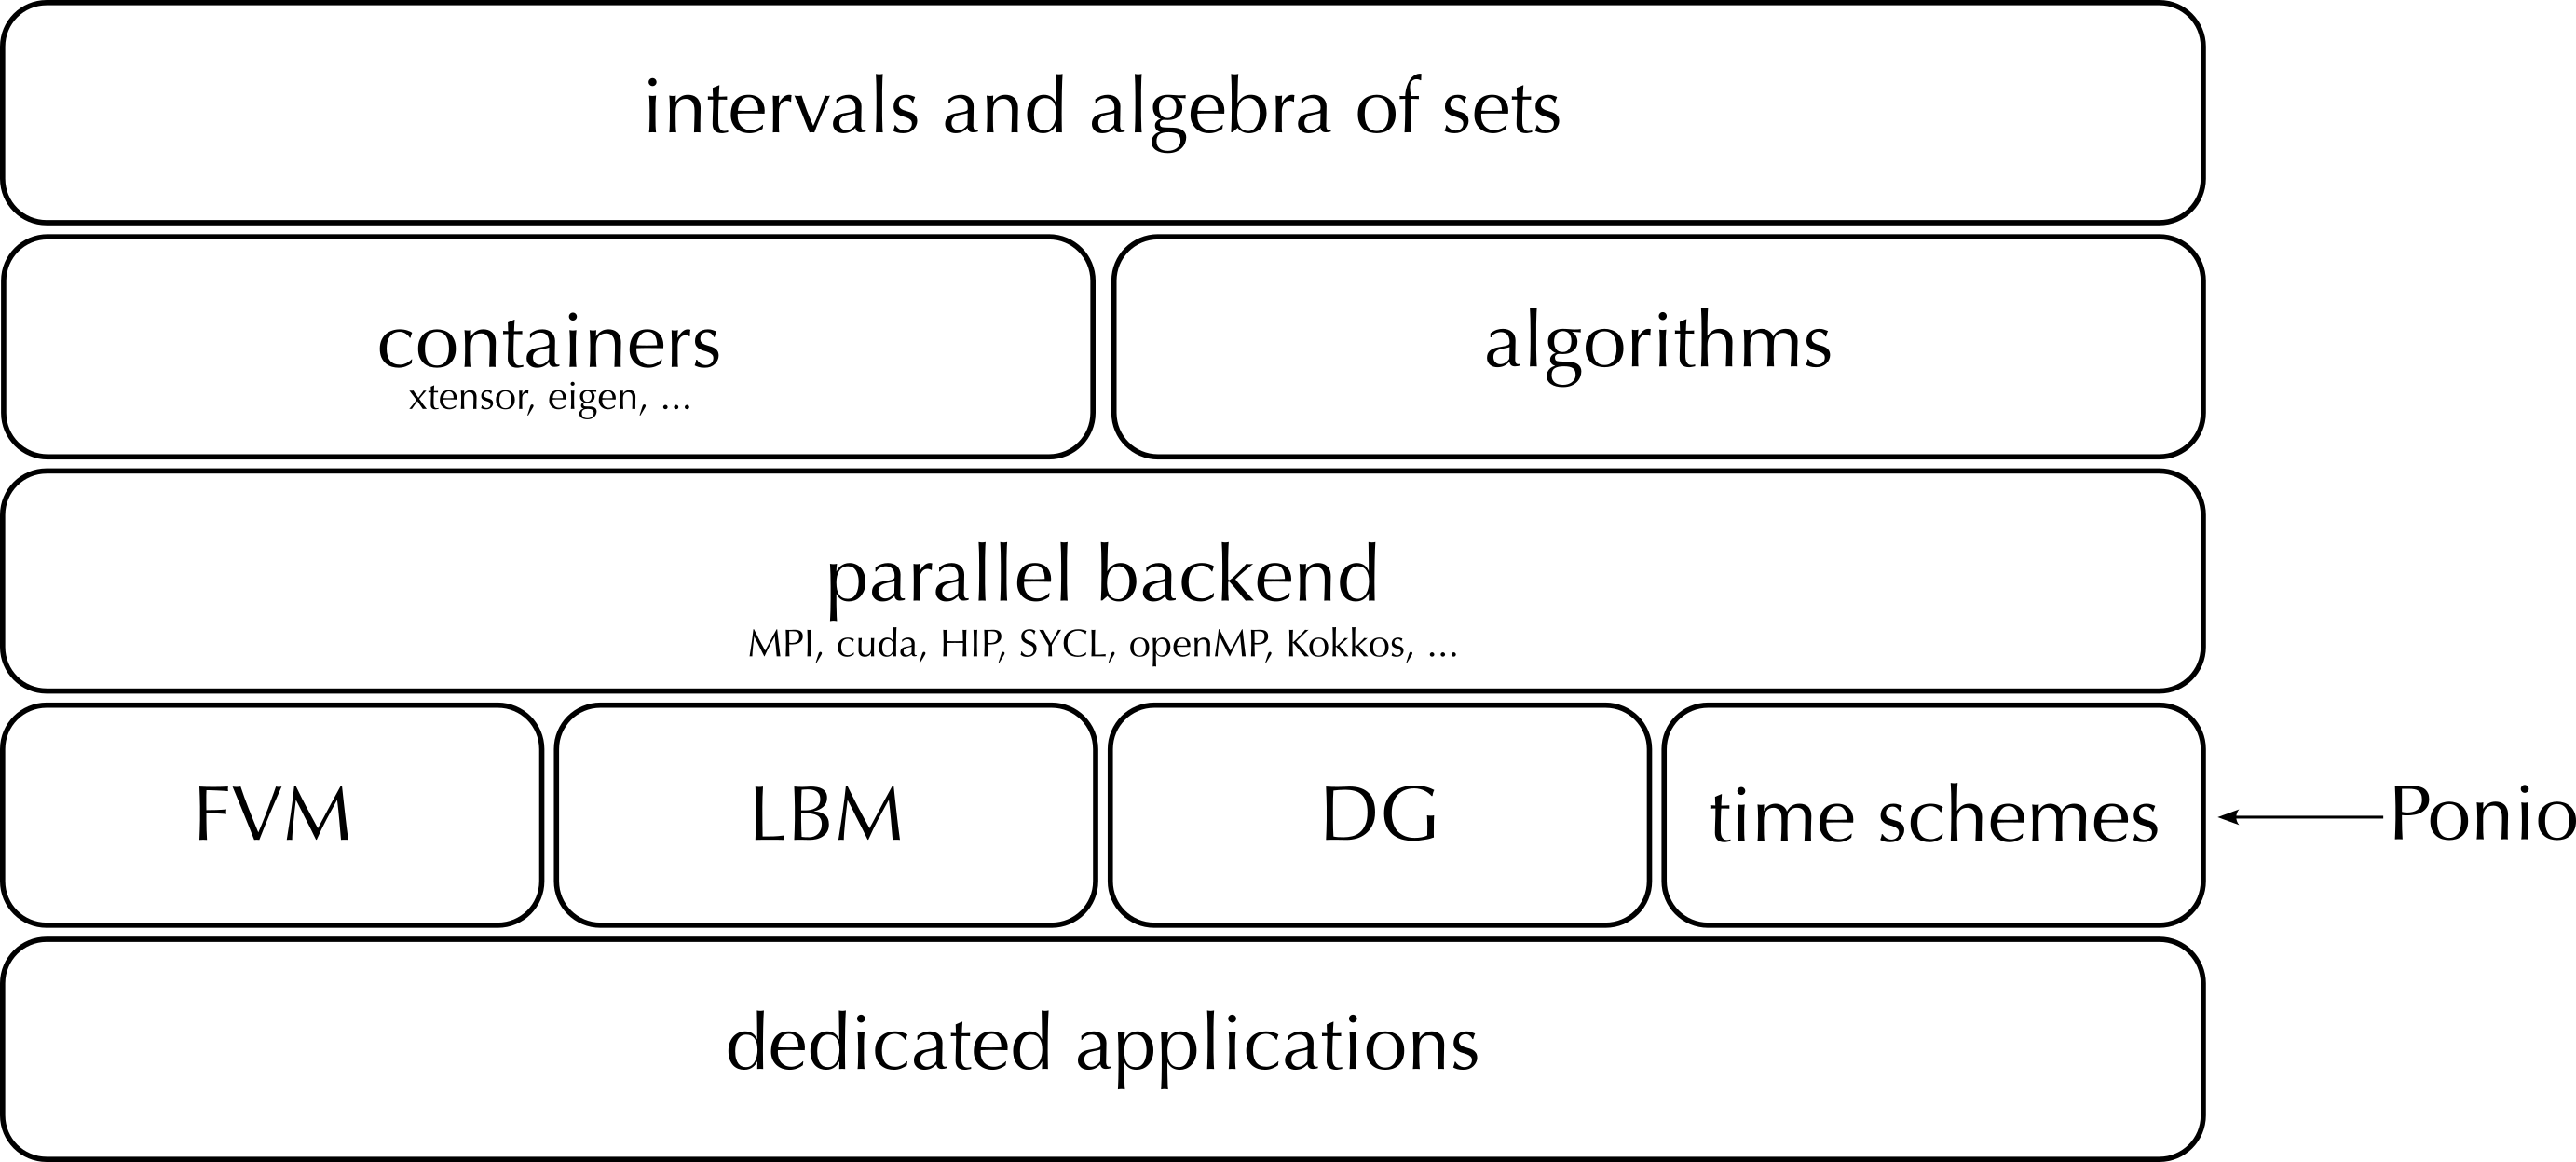
\includegraphics[width=0.8\textwidth]{graphics/samurai/samurai.png}
    \caption{Samurai architecture}
    \label{fig:Samurai:architecture}
\end{figure}

\href{https://github.com/hpc-maths/ponio}{ponio} is an open source software developed at the HPC@Maths team at CMAP (Ecole polytechnique). The aim of ponio is to provide a set of schemes in time for solving a whole collection of ODEs and PDEs. The simplest is the combination of an operator separation strategy and a method of line involving various classical time integrators like Runge-Kutta methods, or optimized ones (RADAU5, ROCK4) and also operator splitting methods as well as IMEX schemes; the long-term objective is also to be able to tackle innovative adaptive code coupling techniques through an interface as well as classes of time-space coupled schemes (Lax-Wendroff, OSMP, time-space coupled IMEX with good asymptotic preserving and stability properties...).

The design principles of samurai are the following:
\begin{enumerate}
    \item Compress the mesh according to the level-wise spatial connectivity along each Cartesian axis.
    \item Achieve fast look-up for a cell into the structure, especially for parents and neighbors. This is particularly useful when utilizing numerical schemes such as Finite Volumes, \emph{etc.} on the hybrid mesh.
    \item Maximize the memory contiguity of the stored data to allow for caching and vectorization (contrarily to the $z$-curve).
    \item Facilitate inter-level operations which are common in many numerical techniques (\emph{e.g.} multiresolution).
    \item Allow for a time evolution of the hybrid mesh (\emph{via} AMR or multiresolution)  efficiently.
    \item Give the possibility of writing numerical schemes in a transparent way as one were on a uniform mesh.
\end{enumerate}

To give an overview of the compression capabilities of samurai, the~\cref{tab:Samurai:compression} shows the number of cells needed to represent a Cartesian mesh defined by the simple-2d example found in the p4est library (\cite{burstedde_p4est_2011}) and illustrated in~\cref{fig:Samurai:simple2d}.

\begin{figure}[h!]
    \centering
    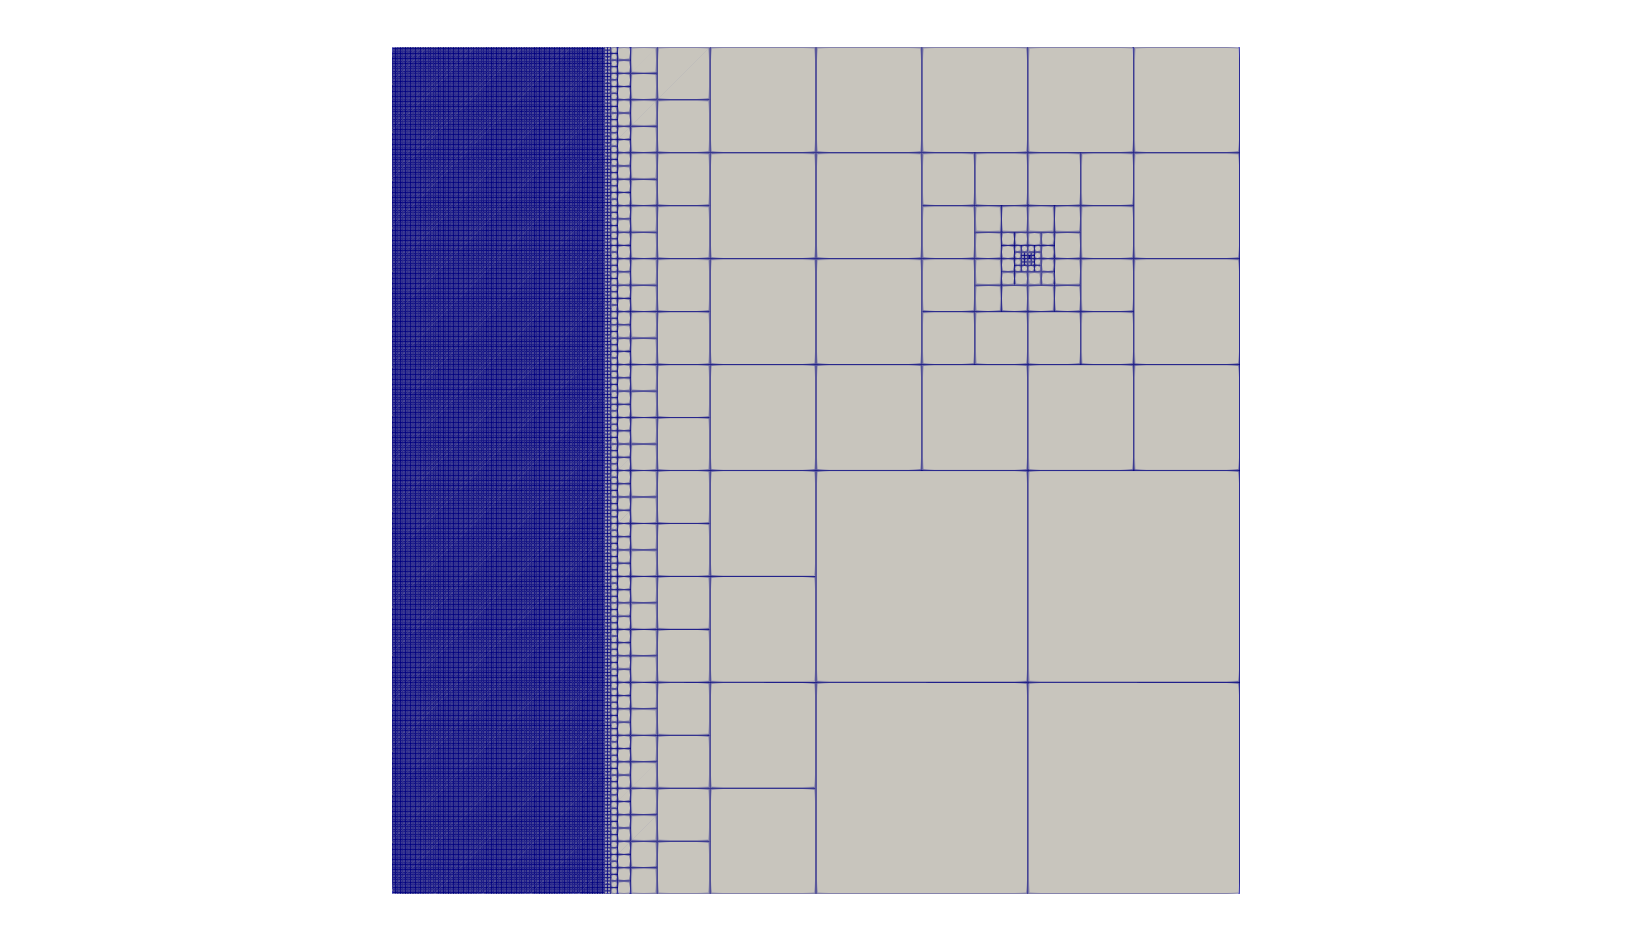
\includegraphics[width=0.8\textwidth]{graphics/samurai/p4est_3.png}
    \caption{simple-2d test from p4est library}
    \label{fig:Samurai:simple2d}
\end{figure}

\begin{table}[h!]
    \centering
    {
        \setlength{\parindent}{0pt}
        \def\arraystretch{1.25}
        \arrayrulecolor{numpexgray}
        {
            \fontsize{9}{11}\selectfont
            \begin{tabular}{llllll}

    \rowcolor{numpexgray}{\rule{0pt}{2.5ex}\color{white}\bf Level} &  {\rule{0pt}{2.5ex}\color{white}\bf Num. of cells }  &{\rule{0pt}{2.5ex}\color{white}\bf p4est} &  {\rule{0pt}{2.5ex}\color{white}\bf samurai (leaves) } &{\rule{0pt}{2.5ex}\color{white}\bf samurai (all)} &  {\rule{0pt}{2.5ex}\color{white}\bf ratio }\\

    \rowcolor{white} 9 & 66379 & 2.57 Mb & 33.68 Kb & 121 Kb & 21.24 \\
    \rowcolor{numpexlightergray} 10 & 263767 & 10.25 Mb & 66.64 Kb & 236.8 Kb & 43.28 \\
    \rowcolor{white} 11 & 1051747 & 40.96 Mb & 132.36 Kb & 467.24 Kb & 87.66 \\
    \rowcolor{numpexlightergray} 12 & 4200559 & 163.75 Mb & 263.6 Kb & 927 Kb & 176.64 \\
    \rowcolor{white} 13 & 16789627 & 654.86 Mb & 525.9 Kb & 1.85 Mb & 353.98 \\
    \rowcolor{numpexlightergray} 14 & 67133575 & 2.61 Gb & 1.05 Mb & 3.68 Mb & 709.24 \\
\end{tabular}
        }
    }
    \caption{WP1: Compression rate between samurai and p4est meshes}
    \label{tab:Samurai:compression}
\end{table}

\subsection{Purpose}
\label{sec:Samurai:purpose}

Based on this new data structure, samurai's objective is to be able to easily describe AMR mesh adaptation methods with a heuristic refinement criterion, or multiresolution methods based on a wavelet base decomposition (\cite{cohen_fully_2003}). Multiresolution, although more complicated to implement, offers greater robustness than AMR methods, since the refinement criterion is based solely on the calculation of a detail derived from the wavelet decomposition. It therefore provides finer control over the error made between the fine solution everywhere and the adapted solution whatever the physical problem studied. Most of available software are based on AMR methods (AMReX \cite{zhang_amrex_2021}, Dyablo \cite{delorme_novel_nodate} and others , \cite{dubey_survey_2014-1}). Only few of them are based on multiresolution methods (Murphy \cite{gillis_murphy---scalable_2022}, Wabbit \cite{krah_wavelet_2022}) and used cell-based structure.

Block-based AMR methods have good memory contiguity thanks to their patch-based hierarchical data structure. This makes it possible to use the vectorization of modern processors. However, to be effective, the patches need to be large enough. It is therefore possible to refine more than necessary.

Cell-based AMR methods lose this memory contiguity, as the mesh is now flattened. A tree-like data structure is therefore required. To restore good arithmetic intensity, it is customary to place cell blocks in the tree leaves. Here again, we refine more than is necessary.

In comparison, the samurai data structure maintains memory contiguity in one direction by using intervals. This is the same as with AMR block-based methods. This ensures that modern processors remain vectorized. What's more, the data structure allows refinement only where necessary. This means no more refinement than is necessary, while maintaining good arithmetic intensity. samurai therefore combines the advantages of the two previous data structures.

\subsection{Programming and Computational Environment}
\label{sec::Samurai:environment_capabilities}


The following table summarizes these aspects for Samurai, providing a  view of its programming and computational capabilities.

\begin{table}[h!]
    \centering
    {
    \setlength{\parindent}{0pt}
    \def\arraystretch{1.25}
    \arrayrulecolor{numpexgray}
    {\fontsize{9}{11}\selectfont
    \begin{tabular}{lp{.3\textwidth}p{.5\textwidth}}
        \rowcolor{numpexgray}{\rule{0pt}{2.5ex}\color{white}\bf Category}  & {\rule{0pt}{2.5ex}\color{white}\bf Details} & {\rule{0pt}{2.5ex}\color{white}\bf Description}\\
        \rowcolor{white}Languages  & \begin{tabular}{l}
C++17\\
\end{tabular} & samurai is developed in modern C++. The source code is written in C++17 but some new implementations will use concepts and ranges provided by C++20.  \\
        \rowcolor{numpexlightergray}Parallelism  & \begin{tabular}{l}
MPI\\
Multithread\\
\end{tabular} & samurai is parallelized using MPI and OpenMP. Kokkos will also be used in future versions to provide GPU support.\\
        \rowcolor{white}Data Formats  & \begin{tabular}{l}
HDF5\\
\end{tabular} & Output is in HDF5 format using the open source software HighFive. Adios2 is another solution being considered for future versions.\\
        \rowcolor{numpexlightergray}Resilience  & \begin{tabular}{l}
None\\
\end{tabular} & There are no fault tolerance and recovery mechanisms used by samurai.\\
        \rowcolor{white}DevOps & \begin{tabular}{l}
Continuous Delivery\\
Continuous Integration\\
\end{tabular} & samurai uses GitHub Actions to perform automatic tasks: documentation build, CI, new releases, etc.  \\
        \rowcolor{numpexlightergray}Packaging  & \begin{tabular}{l}
Other\\
\end{tabular} & samurai is available on conda and conan.\\
        \rowcolor{white}Testing  & \begin{tabular}{l}
Functional\\
Unit\\
Validation\\
Verification\\
\end{tabular} & samurai has unit tests and regression tests. All the examples provided by samurai in its demos directory are verified at every change of the code.\\
        \rowcolor{numpexlightergray}Containerization  & \begin{tabular}{l}
None\\
\end{tabular} & No container technologies are used to package and deploy the software. We use conda-forge to built the conda package.\\
        \rowcolor{white}Interfaces  & \begin{tabular}{l}
PETSc\\
xtensor\\
Eigen\\
\end{tabular} & xtensor and Eigen are used to store the unknowns of the equations and to perform lazy evaluation. Matrix assembly and linear solver resolution are performed using PETSc.\\
        \bottomrule
    \end{tabular}
    }}
    \caption{Samurai programming and computational environment}
\end{table}



\subsection{Mathematics}
\label{sec:Samurai:mathematics}

samurai provides a set of operators for working with Cartesian grids of varying resolutions. Two distinct categories of operators can be identified:

\begin{itemize}
\item Prediction operators are employed to calculate the value of a field on a fine grid based on the value of a field on a coarse grid.
\item Projection operators are used to determine the value of a field on a coarse grid by using the value of a field on a fine grid.
\end{itemize}

The aforementioned operators are currently defined for control volumes up to order 11. The size of the associated stencils is automatically accounted for by samurai. In a near future, the same operators will be defined for finite differences and discountinuous Galerkin methods.

It is thus possible to reconstruct the solution at any desired resolution level. This enables the solution to be found at the finest level, as well as calculations to be performed involving two different AMR meshes. To illustrate this purpose, we can imagine a case where one mesh is used to solve the Navier-Stokes equations, while another is employed to simulate the propagation of a pollutant via an advection equation, wherein the velocity is derived from the velocity provided by the Navier-Stokes equations. The first mesh is adapted using the velocity field, whereas the second mesh is adapted using the pollutant concentration (\cite{nguessan_high_2021}).

In addition to these resolution-level operators, samurai provides an API for defining finite-volume operators that can be used for both explicit and implicit methods. The defined FVM operator available with samurai are

\begin{itemize}
    \item linear homogeneous operator
    \item linear heterogeneous operator
    \item non-linear operator
\end{itemize}

In the following, we will illustrate the use of samurai with a simple example of a linear homogeneous operator. The operator is a scalar Laplacian operator defined as follows:

Since we have

\begin{equation*}
\int_V \Delta u = \int_{\partial V} \nabla u\cdot \mathbf{n},
\end{equation*}

the flux function to implement is a discrete version of $\nabla u\cdot \mathbf{n}$.
Here, we choose the normal gradient of the first order, requiring a stencil of two cells.
This is enough to write the static configuration:

\begin{listing}[ht]
\begin{minted}[
    linenos,                % Line numbers
    fontsize=\scriptsize,        % Reduce font size
    bgcolor=bgcolor,        % Slightly gray background
    frame=lines,            % Delimiters around the code
    framesep=2mm,           % Space between code and frame
    rulecolor=\color{gray}, % Color of the frame
    breaklines              % Allow line breaks in long lines
  ]{cpp}
auto u = samurai::make_field<1>("u", mesh); // scalar field

using cfg = samurai::FluxConfig<SchemeType::LinearHomogeneous,
                                1,            // output_field_size
                                2,            // stencil_size
                                decltype(u)>; // input_field_type
\end{minted}
\end{listing}

Now, denoting by $V_L$ (left) and $V_R$ (right) the stencil cells and $F$ their interface, the discrete flux from $V_L$ to $V_R$ writes

\begin{equation*}
    \mathcal{F}_h(u_h)_{|F} := \frac{u_R-u_L}{h},
\end{equation*}

where $u_L$ and $u_R$ are the finite volume approximations of $u$ in the respective cells, and $h$ is the cell length.
%Referring to formula :eq:`linear_comb`, the coefficients in the linear combination of $(u_L, u_R)$ correspond to $(-1/h, 1/h)$.
The flux function then writes:

\begin{listing}[ht]
    \begin{minted}[
        linenos,                % Line numbers
        fontsize=\scriptsize,        % Reduce font size
        bgcolor=bgcolor,        % Slightly gray background
        frame=lines,            % Delimiters around the code
        framesep=2mm,           % Space between code and frame
        rulecolor=\color{gray}, % Color of the frame
        breaklines              % Allow line breaks in long lines
      ]{cpp}
samurai::FluxDefinition<cfg> gradient([](double h)
{
    static constexpr std::size_t L = 0; // left
    static constexpr std::size_t R = 1; // right

    samurai::FluxStencilCoeffs<cfg> c;
    c[L] = -1/h;
    c[R] =  1/h;
    return c;
});
\end{minted}
\end{listing}

First of all, remark that we have declared only one flux function for all directions.
We could have written as many functions as directions:
they would have been identical, except that we would have replaced the name of the constants
\verb!L=0, R=1! with \verb!B=0, T=1! (bottom, top) and \verb!B=0, F=1! (back, front) to better reflect the actual direction currently managed.
The indexes 0 and 1 actually refer to the configured stencil.
In this case, no particular stencil has been defined, so the default ones are used: in the x-direction of a 3D space,
it is \verb!{{0,0,0}, {1,0,0}}!, i.e. the current cell at index 0 (which we call \verb!L!) and its right neighbor at index 1 (which we call \verb!R!).

Finally, the operator must be constructed from the flux definition by the instruction

\begin{listing}[ht]
    \begin{minted}[
        linenos,                % Line numbers
        fontsize=\scriptsize,        % Reduce font size
        bgcolor=bgcolor,        % Slightly gray background
        frame=lines,            % Delimiters around the code
        framesep=2mm,           % Space between code and frame
        rulecolor=\color{gray}, % Color of the frame
        breaklines              % Allow line breaks in long lines
      ]{cpp}
auto laplacian = samurai::make_flux_based_scheme(gradient);
\end{minted}
\end{listing}

samurai uses lazy evaluation to have concise and readable equations. The following code snippet shows how to apply the operator to a field to solve the heat equation in implicit and explicit ways using backward Euler time scheme

\begin{listing}[ht]
    \begin{minted}[
        linenos,                % Line numbers
        fontsize=\scriptsize,        % Reduce font size
        bgcolor=bgcolor,        % Slightly gray background
        frame=lines,            % Delimiters around the code
        framesep=2mm,           % Space between code and frame
        rulecolor=\color{gray}, % Color of the frame
        breaklines              % Allow line breaks in long lines
      ]{cpp}
auto unp1 = samurai::make_field<1>("unp1", mesh);
if (explicit_scheme)
{
    unp1 = u - dt * laplacian(u);
}
else
{
    auto back_euler = id + dt * laplacian;
    samurai::petsc::solve(back_euler, unp1, u); // solves the linear equation   [Id + dt*Diff](unp1) = u
}
\end{minted}
\end{listing}

It can be observed that the implicit case is constructed and solved using PETSc.

These operators can then be used in adapted mesh refinement methods.

Other spatial discretization methods will soon be proposed in samurai, such as finite differences and discontinuous Galerkin methods based on the same operator definition approach.

\subsection{Relevant Publications}
\label{sec:Samurai:publications}

Here is a list of relevant publications related to the software:

\begin{itemize}
    \item \cite{bellotti_multidimensional_2022}: this article explains how to use the adaptive multiresolution (MR) approach based on wavelets with lattice Boltzmann methods.
    \item \cite{bellotti_multiresolution-based_2022}: in this article, an error analysis is proposed. For the purpose of validating this error analysis, we conduct a series of test cases for various schemes and scalar and systems of conservation laws, where solutions with shocks are to be found and local mesh adaptation is especially relevant. Theoretical estimates are retrieved while a reduced memory footprint is observed.
\end{itemize}

\subsection{Acknowledgements}
\label{sec::Samurai:acknowledgements}

The software has been developed with the support of the following funding agencies and institutions:
\begin{itemize}
    \item \'Ecole polytechnique
    \item CNRS
    \item CIEDS
 \end{itemize}

\section{Software: Scimba}
\label{sec:Scimba:software}



\begin{table}[h!]
    \centering
    { \setlength{\parindent}{0pt}
        \def\arraystretch{1.25}
        \arrayrulecolor{numpexgray}
        {\fontsize{9}{11}\selectfont
            \begin{tabular}{!{\color{numpexgray}\vrule}p{.4\textwidth}!{\color{numpexgray}\vrule}p{.6\textwidth}!{\color{numpexgray}\vrule}}
                \rowcolor{numpexgray}{\rule{0pt}{2.5ex}\color{white}\bf Field}
                 & {\rule{0pt}{2.5ex}\color{white}\bf Details}                                         \\
                \rowcolor{white}\textbf{Consortium}
                 & \begin{tabular}{l}
                       INRIA   \\
                       UNISTRA \\
                   \end{tabular}                                                                   \\
                \rowcolor{numpexlightergray}\textbf{Exa-MA Partners}
                 & \begin{tabular}{l}
                       Unistra \\
                   \end{tabular}                                                                   \\
                \rowcolor{white}\textbf{Contact Emails}
                 & \begin{tabular}{l}
                       emmanuel.franck@inria.fr      \\
                       victor.michel-dansac@inria.fr \\
                   \end{tabular}                                                       \\
                \rowcolor{numpexlightergray}\textbf{Supported Architectures}
                 & \begin{tabular}{l}
                       CPU or GPU \\
                   \end{tabular}                                                                   \\
                \rowcolor{white}\textbf{Repository}
                 & \href{https://gitlab.inria.fr/scimba/scimba}{https://gitlab.inria.fr/scimba/scimba} \\
                \rowcolor{numpexlightergray}\textbf{License}
                 & \begin{tabular}{l}
                       MIT \\
                   \end{tabular}                                                                   \\
                \rowcolor{white}\textbf{Bottlenecks roadmap}
                 & \begin{tabular}{l}
                       B10 - Scientific Productivity                          \\
                       B11 - Reproducibility and Replicability of Computation \\
                       B6 - Data Management                                   \\
                       B7 - Exascale Algorithms                               \\
                   \end{tabular}                              \\
                \bottomrule
            \end{tabular}
        }}
    \caption{Scimba Information}
\end{table}

\subsection{Software summary}
\label{sec:Scimba:summary}
Detailed overview not available.


\subsection{Purpose}
\label{sec:Scimba:purpose}
Purpose not available.

\subsection{Programming and Computational Environment}
\label{sec::Scimba:environment_capabilities}


The following table summarizes these aspects for Scimba, providing a  view of its programming and computational capabilities.

\begin{table}[h!]
    \centering
    {
        \setlength{\parindent}{0pt}
        \def\arraystretch{1.25}
        \arrayrulecolor{numpexgray}
        {\fontsize{9}{11}\selectfont
            \begin{tabular}{lp{.3\textwidth}p{.5\textwidth}}
                \rowcolor{numpexgray}{\rule{0pt}{2.5ex}\color{white}\bf Category}
                 & {\rule{0pt}{2.5ex}\color{white}\bf Details}
                 & {\rule{0pt}{2.5ex}\color{white}\bf Description}                                                                                   \\
                \rowcolor{white}Languages
                 & \begin{tabular}{l}
                       Python \\
                   \end{tabular}
                 & Programming languages and language standards supported by the software                                                            \\
                \rowcolor{numpexlightergray}Parallelism
                 & \begin{tabular}{l}
                       GPU, CPU (shared) \\
                   \end{tabular}
                 & Parallel computing methods and frameworks utilized by the software.                                                               \\
                \rowcolor{white}Data Formats
                 & \begin{tabular}{l}
                       input: none                          \\
                       output: \texttt{.pth} \& image files \\
                   \end{tabular}
                 & Data formats that the software can handle or produce.                                                                             \\
                \rowcolor{numpexlightergray}Resilience
                 & \begin{tabular}{l}
                       None \\
                   \end{tabular}
                 & Fault tolerance and recovery mechanisms employed by the software.                                                                 \\
                \rowcolor{white}DevOps
                 & \begin{tabular}{l}
                       None \\
                   \end{tabular}
                 & Outlines the development and operational practices including continuous integration, containerization, and testing methodologies. \\
                \rowcolor{numpexlightergray}Packaging
                 & \begin{tabular}{l}
                       pip, GitHub \\
                   \end{tabular}
                 & Software packaging and distribution.                                                                                              \\
                \rowcolor{white}Testing
                 & \begin{tabular}{l}
                       pytest \\
                   \end{tabular}
                 & Testing methodologies employed to ensure software quality and correctness.                                                        \\
                \rowcolor{numpexlightergray}Containerization
                 & \begin{tabular}{l}
                       None \\
                   \end{tabular}
                 & Container technologies used to package and deploy the software.                                                                   \\
                \rowcolor{white}Interfaces
                 & \begin{tabular}{l}
                       pytorch \\
                   \end{tabular}
                 & List of software Scimba has interfaces with.                                                                                      \\
                \bottomrule
            \end{tabular}
        }}
    \caption{Scimba programming and computational environment}
\end{table}


\subsection{Mathematics}
\label{sec:Scimba:mathematics}
% Mathematics not available.

% In this section, provide a summary the mathematics used in the software.

This software mainly uses physics-informed
learning~\cite{KarKevLuPerWanYan2021}
to solve partial differential equations.
More specifically, it solves partial differential equations of the form
\begin{equation*}
    \begin{cases}
        \mathcal{D}(u, x, t,; \mu) = 0,
         & \text{in } \Omega \times (0,T) \times \mathbb{M},          \\
        \mathcal{B}(u, x, t; \mu) = 0,
         & \text{on } \partial \Omega \times (0,T) \times \mathbb{M}, \\
        u(x, 0; \mu) = u_0(x; \mu),
         & \text{on } \Omega \times \mathbb{M},                       \\
    \end{cases}
\end{equation*}
with $\mathcal{D}$ a differential operator, $\mathcal{B}$ a boundary condition operator,
$u_0$ an initial condition, $\Omega$ the spatial domain,
$T$ the final time, and $\mathbb{M}$ the parameter space.
The solution $u$ is approximated with a variety of physics-informed neural networks,
which are trained to minimize the residual of the PDE,
the boundary conditions and the initial conditions.
An example of a physics-informed loss function is:
\begin{equation*}
    \begin{aligned}
    \mathcal{L} & =
    \int_\Omega \int_0^T \int_{\mathbb{M}}
    ||\mathcal{D}(u, x, t; \mu)||^2 \,
    \mathrm{d}\mu \, \mathrm{d}t \, \mathrm{d}x \\
    & +
    \int_{\partial\Omega} \int_0^T \int_{\mathbb{M}}
    ||\mathcal{B}(u, x, t; \mu)||^2 \,
    \mathrm{d}\mu \, \mathrm{d}t \, \mathrm{d}x
    +
    \int_{\Omega} \int_{\mathbb{M}}
    ||u(x, 0; \mu) - u_0(x;\mu)||^2 \,
    \mathrm{d}\mu \, \mathrm{d}x.
    \end{aligned}
\end{equation*}
Other data-driven methods
(e.g. DeepONets~\cite{LuJinPanZhoKar2021})
or numerical methods
(e.g. Neural Galerkin~\cite{BruPehVan2024})
are also available in Scimba.

% \subsection{Relevant Publications}
% \label{sec:Scimba:publications}

% Here is a list of relevant publications related to the software:


\subsection{Acknowledgements}
\label{sec::Scimba:acknowledgements}

Scimba has mainly been developed by Inria research scientists.
Other contributors include students and researchers
from the University of Strasbourg and CEA Cadarache.
For the moment, no specific funding has been dedicated to Scimba.


\section{Software: TRUST Platform}
\label{sec:TRUST Platform:software}



\begin{table}[h!]
    \centering
    { \setlength{\parindent}{0pt}
    \def\arraystretch{1.25}
    \arrayrulecolor{numpexgray}
    {\fontsize{9}{11}\selectfont
    \begin{tabular}{!{\color{numpexgray}\vrule}p{.4\textwidth}!{\color{numpexgray}\vrule}p{.6\textwidth}!{\color{numpexgray}\vrule}}
        \rowcolor{numpexgray}{\rule{0pt}{2.5ex}\color{white}\bf Field} & {\rule{0pt}{2.5ex}\color{white}\bf Details} \\
        \rowcolor{white}\textbf{Consortium} & \begin{tabular}{l}
CEA\\
\end{tabular} \\
        \rowcolor{numpexlightergray}\textbf{Exa-MA Partners} & \begin{tabular}{l}
CEA\\
\end{tabular} \\
        \rowcolor{white}\textbf{Contact Emails} & \begin{tabular}{l}
pierre.ledac@cea.fr\\
\end{tabular} \\
        \rowcolor{numpexlightergray}\textbf{Supported Architectures} & \begin{tabular}{l}
CPU\\
GPU\\
\end{tabular} \\
        \rowcolor{white}\textbf{Repository} & \href{https://github.com/cea-trust-platform}{https://github.com/cea-trust-platform} \\
        \rowcolor{numpexlightergray}\textbf{License} & \begin{tabular}{l}
OSS::\\
OSS::BSD\\
\end{tabular} \\
        \bottomrule
    \end{tabular}
    }}
    \caption{TRUST Platform Information}
\end{table}

\subsection{Software summary}
\label{sec:TRUST Platform:summary}
Detailed overview not available.



\subsection{Purpose}
\label{sec:TRUST Platform:purpose}
Purpose not available.

\subsection{Programming and Computational Environment}
\label{sec::TRUST Platform:environment_capabilities}


The following table summarizes these aspects for TRUST Platform, providing a  view of its programming and computational capabilities.

\begin{table}[h!]
    \centering
    {
    \setlength{\parindent}{0pt}
    \def\arraystretch{1.25}
    \arrayrulecolor{numpexgray}
    {\fontsize{9}{11}\selectfont
    \begin{tabular}{lp{.3\textwidth}p{.5\textwidth}}
        \rowcolor{numpexgray}{\rule{0pt}{2.5ex}\color{white}\bf Category}  & {\rule{0pt}{2.5ex}\color{white}\bf Details} & {\rule{0pt}{2.5ex}\color{white}\bf Description}\\
        \rowcolor{white}Languages  & \begin{tabular}{l}
C++\\
\end{tabular} & Programming languages and language standards supported by the software \\
        \rowcolor{numpexlightergray}Parallelism  & \begin{tabular}{l}
GPU\\
MPI\\
\end{tabular} & Parallel computing methods and frameworks utilized by the software.\\
        \rowcolor{white}Data Formats  & \begin{tabular}{l}
HDF5\\
MED\\
VTK\\
in-house format\\
\end{tabular} & Data formats that the software can handle or produce.\\
        \rowcolor{numpexlightergray}Resilience  & \begin{tabular}{l}
Checkpoint restart\\
\end{tabular} & Fault tolerance and recovery mechanisms employed by the software.\\
        \rowcolor{white}DevOps & \begin{tabular}{l}
Continuous Integration\\
\end{tabular} & Outlines the development and operational practices including continuous integration, containerization, and testing methodologies.  \\
        \rowcolor{numpexlightergray}Packaging  & \begin{tabular}{l}
None\\
\end{tabular} & Software packaging and distribution.\\
        \rowcolor{white}Testing  & \begin{tabular}{l}
Unit\\
Verification\\
\end{tabular} & Testing methodologies employed to ensure software quality and correctness.\\
        \rowcolor{numpexlightergray}Containerization  & \begin{tabular}{l}
None\\
\end{tabular} & Container technologies used to package and deploy the software.\\
        \rowcolor{white}Interfaces  & \begin{tabular}{l}
None\\
\end{tabular} & List of software TRUST Platform has interfaces with.\\
        \bottomrule
    \end{tabular}
    }}
    \caption{TRUST Platform programming and computational environment}
\end{table}



\subsection{Mathematics}
\label{sec:TRUST Platform:mathematics}
Mathematics not available.

In this section, provide a summary the mathematics used in the software.


\subsection{Relevant Publications}
\label{sec:TRUST Platform:publications}

Here is a list of relevant publications related to the software:


\subsection{Acknowledgements}
\label{sec::TRUST Platform:acknowledgements}

The software has been developed with the support of the following funding agencies and institutions: 




Acknowledgements not available.



\section{Software: Uranie}
\label{sec:Uranie:software}



\begin{table}[ht!]
    \centering
    { \setlength{\parindent}{0pt}
    \def\arraystretch{1.25}
    \arrayrulecolor{numpexgray}
    {\fontsize{9}{11}\selectfont
    \begin{tabular}{!{\color{numpexgray}\vrule}p{.4\textwidth}!{\color{numpexgray}\vrule}p{.6\textwidth}!{\color{numpexgray}\vrule}}
        \rowcolor{numpexgray}{\rule{0pt}{2.5ex}\color{white}\bf Field} & {\rule{0pt}{2.5ex}\color{white}\bf Details} \\
        \rowcolor{white}\textbf{Consortium} & \begin{tabular}{l}
CEA\\
\end{tabular} \\
        \rowcolor{numpexlightergray}\textbf{Exa-MA Partners} & \begin{tabular}{l}
CEA\\
\end{tabular} \\
        \rowcolor{white}\textbf{Contact Emails} & \begin{tabular}{l}
clement.gauchy@cea.fr\\
jean-baptiste.blanchard@cea.fr\\
rudy.chocat@cea.fr\\
\end{tabular} \\
        \rowcolor{numpexlightergray}\textbf{Supported Architectures} & \begin{tabular}{l}
CPU, GPU\\
\end{tabular} \\
        \rowcolor{white}\textbf{Repository} & \href{https://uranie.cea.fr}{https://uranie.cea.fr} \\
        \rowcolor{numpexlightergray}\textbf{License} & \begin{tabular}{l}
OSS:: LGPL \\
\end{tabular} \\
        \rowcolor{white}\textbf{Bottlenecks roadmap} & \begin{tabular}{l}
None\\
\end{tabular} \\
        \bottomrule
    \end{tabular}
    }}
    \caption{Uranie Information}
\end{table}

\subsection{Software summary}
\label{sec:Uranie:summary}

Uranie platform is based on ROOT and has by consequence a lot of ROOT characteristics such as:
\begin{itemize}
    \item Interactive C++ interpreter (Cling) based on LLVM and Clang
    \item Python interface (PyROOT)
    \item SQL database access
\end{itemize}


\subsection{Purpose}
\label{sec:Uranie:purpose}

Uranie (the version under discussion here being v4.9.0) is a software dedicated to perform studies on uncertainty propagation, sensitivity analysis and surrogate model generation and calibration, based on ROOT (the corresponding version being v6.32.00). The motivation for the development of Uranie is the VVUQ (Verification, Validation and Uncertainty Quantification) approach for conceiving a numerical model of real physical phenomena of interests. Uranie is developed such that it interfaces well with CEA internal numerical simulation software.


\begin{table}[ht!]
    \centering
    {
    \setlength{\parindent}{0pt}
    \def\arraystretch{1.25}
    \arrayrulecolor{numpexgray}
    {\fontsize{9}{11}\selectfont
    \begin{tabular}{lp{.3\textwidth}p{.5\textwidth}}
        \rowcolor{numpexgray}{\rule{0pt}{2.5ex}\color{white}\bf Category}  & {\rule{0pt}{2.5ex}\color{white}\bf Details} & {\rule{0pt}{2.5ex}\color{white}\bf Description}\\
        \rowcolor{white}Languages  & \begin{tabular}{l}
C++\\
Python\\
\end{tabular} & Programming languages and language standards supported by the software \\
        \rowcolor{numpexlightergray}Parallelism  & \begin{tabular}{l}
GPU\\
MPI\\
Multithread\\
\end{tabular} & Parallel computing methods and frameworks utilized by the software.\\
        \rowcolor{white}Data Formats  & \begin{tabular}{l}
SALOME format\\
ROOT\\
SQL\\
\end{tabular} & Data formats that the software can handle or produce.\\
        \rowcolor{numpexlightergray}Resilience  & \begin{tabular}{l}
None\\
\end{tabular} & Fault tolerance and recovery mechanisms employed by the software.\\
        \rowcolor{white}DevOps & \begin{tabular}{l}
Continuous Integration\\
\end{tabular} & Outlines the development and operational practices including continuous integration, containerization, and testing methodologies.  \\
        \rowcolor{numpexlightergray}Packaging  & \begin{tabular}{l}
None\\
\end{tabular} & Software packaging and distribution.\\
        \rowcolor{white}Testing  & \begin{tabular}{l}
Unit\\
Validation\\
Verification\\
\end{tabular} & Testing methodologies employed to ensure software quality and correctness.\\
        \rowcolor{numpexlightergray}Containerization  & \begin{tabular}{l}
None\\
\end{tabular} & Container technologies used to package and deploy the software.\\
        \rowcolor{white}Interfaces  & \begin{tabular}{l}
Salome \\
Trust \\
\end{tabular} & List of software Uranie has interfaces with.\\
        \bottomrule
    \end{tabular}
    }}
    \caption{Uranie programming and computational environment}
\end{table}


\subsection{Application entry points}
\label{sec:Uranie:apps}
Uranie is used as the VVUQ and calibration backbone for several activities; see Chapter~\ref{chap:applications}:
\begin{itemize}
        \item Ensemble Kalman Inversion (calibration and UQ, proposed): Section~\ref{sec:app:specs:app-eki}.
\end{itemize}



\subsection{Mathematics}
\label{sec:Uranie:mathematics}
The mathematics used in Uranie are related to:
\begin{itemize}
        \item Surrogate modeling \& machine learning techniques: Gaussian process regression, neural networks, polynomial chaos expansion
        \item Optimization: EGO-like algorithm and ants colony based metaheuristics
        \item Calibration: Latent parameters estimations \& Bayesian algorithms
        \item Sensitivity analysis: HSIC indices estimation, Sobol' indices.
\end{itemize}


\subsection{Relevant Publications}
\label{sec:Uranie:publications}

Here is a relevant publication used to cite Uranie:

\begin{itemize}
   \item \fullcite{blanchard_uranie_2019}
\end{itemize}


\subsection{Acknowledgements}
\label{sec::Uranie:acknowledgements}

The software has been developed in \href{https://www.cea.fr/}{CEA} and funded by the SIMU research program.




\section{Software: Zellij}
\label{sec:Zellij:software}



\begin{table}[h!]
    \centering
    { \setlength{\parindent}{0pt}
    \def\arraystretch{1.25}
    \arrayrulecolor{numpexgray}
    {\fontsize{9}{11}\selectfont
    \begin{tabular}{!{\color{numpexgray}\vrule}p{.4\textwidth}!{\color{numpexgray}\vrule}p{.6\textwidth}!{\color{numpexgray}\vrule}}
        \rowcolor{numpexgray}{\rule{0pt}{2.5ex}\color{white}\bf Field} & {\rule{0pt}{2.5ex}\color{white}\bf Details} \\
        \rowcolor{white}\textbf{Consortium} & \begin{tabular}{l}
Université de Lille\\
\end{tabular} \\
        \rowcolor{numpexlightergray}\textbf{Exa-MA Partners} & \begin{tabular}{l}
Inria Lille\\
\end{tabular} \\
        \rowcolor{white}\textbf{Contact Emails} & \begin{tabular}{l}
el-ghazali.talbi@univ-lille.fr\\
\end{tabular} \\
        \rowcolor{numpexlightergray}\textbf{Supported Architectures} & \begin{tabular}{l}
GPU Only\\
\end{tabular} \\
        \rowcolor{white}\textbf{Repository} & \href{https://github.com/ThomasFirmin/zellij}{https://github.com/ThomasFirmin/zellij} \\
        \rowcolor{numpexlightergray}\textbf{License} & \begin{tabular}{l}
OSS: Cecill-*\\
\end{tabular} \\
        \rowcolor{white}\textbf{Bottlenecks roadmap} & \begin{tabular}{l}
B10 - Scientific Productivity\\
B11 - Reproducibility and Replicability of Computation\\
B6 - Data Management\\
B7 - Exascale Algorithms\\
\end{tabular} \\
        \bottomrule
    \end{tabular}
    }}
    \caption{Zellij Information}
\end{table}

\subsection{Software summary}
\label{sec:Zellij:summary}
Detailed overview not available.



\subsection{Purpose}
\label{sec:Zellij:purpose}
Purpose not available.

\subsection{Programming and Computational Environment}
\label{sec::Zellij:environment_capabilities}


The following table summarizes these aspects for Zellij, providing a  view of its programming and computational capabilities.

\begin{table}[h!]
    \centering
    {
    \setlength{\parindent}{0pt}
    \def\arraystretch{1.25}
    \arrayrulecolor{numpexgray}
    {\fontsize{9}{11}\selectfont
    \begin{tabular}{lp{.3\textwidth}p{.5\textwidth}}
        \rowcolor{numpexgray}{\rule{0pt}{2.5ex}\color{white}\bf Category}  & {\rule{0pt}{2.5ex}\color{white}\bf Details} & {\rule{0pt}{2.5ex}\color{white}\bf Description}\\
        \rowcolor{white}Languages  & \begin{tabular}{l}
Python\\
\end{tabular} & Programming languages and language standards supported by the software \\
        \rowcolor{numpexlightergray}Parallelism  & \begin{tabular}{l}
MPI\\
\end{tabular} & Parallel computing methods and frameworks utilized by the software.\\
        \rowcolor{white}Data Formats  & \begin{tabular}{l}
None\\
\end{tabular} & Data formats that the software can handle or produce.\\
        \rowcolor{numpexlightergray}Resilience  & \begin{tabular}{l}
Checkpoint restart\\
\end{tabular} & Fault tolerance and recovery mechanisms employed by the software.\\
        \rowcolor{white}DevOps & \begin{tabular}{l}
None\\
\end{tabular} & Outlines the development and operational practices including continuous integration, containerization, and testing methodologies.  \\
        \rowcolor{numpexlightergray}Packaging  & \begin{tabular}{l}
None\\
\end{tabular} & Software packaging and distribution.\\
        \rowcolor{white}Testing  & \begin{tabular}{l}
None\\
\end{tabular} & Testing methodologies employed to ensure software quality and correctness.\\
        \rowcolor{numpexlightergray}Containerization  & \begin{tabular}{l}
None\\
\end{tabular} & Container technologies used to package and deploy the software.\\
        \rowcolor{white}Interfaces  & \begin{tabular}{l}
None\\
\end{tabular} & List of software Zellij has interfaces with.\\
        \bottomrule
    \end{tabular}
    }}
    \caption{Zellij programming and computational environment}
\end{table}



\subsection{Mathematics}
\label{sec:Zellij:mathematics}
Mathematics not available.

In this section, provide a summary the mathematics used in the software.


\subsection{Relevant Publications}
\label{sec:Zellij:publications}

Here is a list of relevant publications related to the software:


\subsection{Acknowledgements}
\label{sec::Zellij:acknowledgements}

The software has been developed with the support of the following funding agencies and institutions: 




Acknowledgements not available.




\section{Frameworks to Applications Mapping (Overview)}
This section summarizes how frameworks are used to construct applications as per Chapter~\ref{chap:methodology} and Chapter~\ref{chap:applications}. Detailed specifications remain in Chapter~\ref{chap:applications}.

\begin{itemize}
    \item \textbf{Feel++} → mini‑apps (reduced basis, I/O), demonstrators (thermal, CFD); see Sections on app‑feelpp‑rb, app‑feelpp‑io.
    \item \textbf{HPDDM} → solver kernels for demonstrators and proxy‑apps (domain decomposition preconditioning).
    \item \textbf{FreeFEM++} → extended mini‑apps (mesh adaptation with ParMMG), rapid inverse‑problem templates.
    \item \textbf{CGAL} → geometry/meshing utilities in mini‑apps (wrapping, AABB trees).
    \item \textbf{SciMba/PyTorch} → surrogates for WP2 integrated into demonstrators (multi‑fidelity modeling).
    \item \textbf{TRUST} → CPU+GPU demonstrators.
    \item \textbf{Uranie} → UQ workflows supporting demonstrators and proxy‑apps.
    \item \textbf{Zellij} → optimization engines inside WP5 demonstrators.
\end{itemize}

This mapping is non‑exhaustive and will expand as additional applications mature.

